\documentclass[review]{vgtc}

\graphicspath{{figures/}{pictures/}{images/}{./}}

% Keep the VR template's metrics and line spacing; only add Unicode/CJK fonts.
\usepackage{times}
\renewcommand*\ttdefault{txtt}
\usepackage{mathptmx}
\usepackage{fontspec}
\usepackage{xeCJK}
\setmainfont{Times New Roman}
\setsansfont{Arial}
\setmonofont{Courier New}
\setCJKmainfont[BoldFont=SimHei,ItalicFont=KaiTi]{SimSun}
\setCJKsansfont{Microsoft YaHei}
\setCJKmonofont{FangSong}

\usepackage{amsmath}
\usepackage{amssymb}
\usepackage{array}
\usepackage{booktabs}
\usepackage{multirow}
\usepackage{tabularx}
\usepackage{xcolor}

% EGOANCHOR-EXP-DATA:BEGIN
% Source CSV SHA-256: 215bc4b9f6151d21df8a5bc990a6a0a9ab726c3eaed1fcc4fad3deacba1c9074; Stage 3 TeX SHA-256: bc31c3daceddffe1e73abba388e86cb4e226fba34f1d902b3f42ad3d0a9caf13; generator: egoanchor.eval.materialize-v1; file: exp1_numbers.tex
% Source CSV SHA-256: 215bc4b9f6151d21df8a5bc990a6a0a9ab726c3eaed1fcc4fad3deacba1c9074; Stage 3 TeX SHA-256: 1a9d4754454c36d5b58b03e1232e22cd646973895a14ee1e24bb98a549206f62; generator: egoanchor.eval.materialize-v1; file: exp2_numbers.tex
% 由 egoanchor.eval 自动生成，请勿手工修改本区块。
\newcommand{\EAExpOneArrivalHoldContinuousRotationAngularLagResidualDeg}{2.917}
\newcommand{\EAExpOneArrivalHoldContinuousRotationContinuousRotationPNinetyFiveDeg}{16.848}
\newcommand{\EAExpOneArrivalHoldContinuousRotationDisplayCoveragePct}{100}
\newcommand{\EAExpOneArrivalHoldContinuousRotationEffectiveAngularLagMs}{265}
\newcommand{\EAExpOneArrivalHoldContinuousRotationJumpPNinetyFiveDeg}{3.743}
\newcommand{\EAExpOneArrivalHoldContinuousRotationJumpPNinetyFiveMm}{2.947}
\newcommand{\EAExpOneArrivalHoldContinuousRotationJumpPNinetyNineDeg}{6.897}
\newcommand{\EAExpOneArrivalHoldContinuousRotationJumpPNinetyNineMm}{5.377}
\newcommand{\EAExpOneArrivalHoldContinuousRotationOutputCoveragePct}{100}
\newcommand{\EAExpOneArrivalHoldContinuousTranslationContinuousTranslationPNinetyFiveMm}{73.364}
\newcommand{\EAExpOneArrivalHoldContinuousTranslationDisplayCoveragePct}{100}
\newcommand{\EAExpOneArrivalHoldContinuousTranslationEffectiveTranslationLagMs}{182.5}
\newcommand{\EAExpOneArrivalHoldContinuousTranslationJumpPNinetyFiveDeg}{2.339}
\newcommand{\EAExpOneArrivalHoldContinuousTranslationJumpPNinetyFiveMm}{28.106}
\newcommand{\EAExpOneArrivalHoldContinuousTranslationJumpPNinetyNineDeg}{3.757}
\newcommand{\EAExpOneArrivalHoldContinuousTranslationJumpPNinetyNineMm}{39.498}
\newcommand{\EAExpOneArrivalHoldContinuousTranslationOutputCoveragePct}{100}
\newcommand{\EAExpOneArrivalHoldContinuousTranslationTranslationLagResidualMm}{10.568}
\newcommand{\EAExpOneArrivalHoldOcclusionRecoveryDisplayCoveragePct}{100}
\newcommand{\EAExpOneArrivalHoldOcclusionRecoveryDurableRecoverySuccessPct}{100}
\newcommand{\EAExpOneArrivalHoldOcclusionRecoveryDurableRecoveryTimeMs}{207.577}
\newcommand{\EAExpOneArrivalHoldOcclusionRecoveryFreshOutputTimeMs}{207.577}
\newcommand{\EAExpOneArrivalHoldOcclusionRecoveryJumpPNinetyFiveDeg}{1.521}
\newcommand{\EAExpOneArrivalHoldOcclusionRecoveryJumpPNinetyFiveMm}{0.848}
\newcommand{\EAExpOneArrivalHoldOcclusionRecoveryJumpPNinetyNineDeg}{3.537}
\newcommand{\EAExpOneArrivalHoldOcclusionRecoveryJumpPNinetyNineMm}{4.706}
\newcommand{\EAExpOneArrivalHoldOcclusionRecoveryOcclusionErrorUpdateCount}{13}
\newcommand{\EAExpOneArrivalHoldOcclusionRecoveryOcclusionRotationPNinetyFiveDeg}{24.402}
\newcommand{\EAExpOneArrivalHoldOcclusionRecoveryOcclusionTranslationPNinetyFiveMm}{35.303}
\newcommand{\EAExpOneArrivalHoldOcclusionRecoveryOutputCoveragePct}{82.011}
\newcommand{\EAExpOneArrivalHoldStartStopSixDofDisplayCoveragePct}{100}
\newcommand{\EAExpOneArrivalHoldStartStopSixDofJumpPNinetyFiveDeg}{1.369}
\newcommand{\EAExpOneArrivalHoldStartStopSixDofJumpPNinetyFiveMm}{1.961}
\newcommand{\EAExpOneArrivalHoldStartStopSixDofJumpPNinetyNineDeg}{5.266}
\newcommand{\EAExpOneArrivalHoldStartStopSixDofJumpPNinetyNineMm}{17.517}
\newcommand{\EAExpOneArrivalHoldStartStopSixDofMotionTranslationPNinetyFiveMm}{48.343}
\newcommand{\EAExpOneArrivalHoldStartStopSixDofMotionTranslationPeakMm}{66.636}
\newcommand{\EAExpOneArrivalHoldStartStopSixDofOutputCoveragePct}{100}
\newcommand{\EAExpOneArrivalHoldStartStopSixDofSettlingTimeMs}{0}
\newcommand{\EAExpOneArrivalHoldStartStopSixDofStartStopRotationPNinetyFiveDeg}{23.997}
\newcommand{\EAExpOneArrivalHoldStartStopSixDofVisibleResponseMs}{126.344}
\newcommand{\EAExpOneArrivalHoldStaticHeadMotionAbsoluteTranslationMedianMm}{8.999}
\newcommand{\EAExpOneArrivalHoldStaticHeadMotionDisplayCoveragePct}{100}
\newcommand{\EAExpOneArrivalHoldStaticHeadMotionJumpPNinetyFiveDeg}{1.364}
\newcommand{\EAExpOneArrivalHoldStaticHeadMotionJumpPNinetyFiveMm}{3.975}
\newcommand{\EAExpOneArrivalHoldStaticHeadMotionJumpPNinetyNineDeg}{2.291}
\newcommand{\EAExpOneArrivalHoldStaticHeadMotionJumpPNinetyNineMm}{10.61}
\newcommand{\EAExpOneArrivalHoldStaticHeadMotionOutputCoveragePct}{100}
\newcommand{\EAExpOneArrivalHoldStaticHeadMotionPositionDriftMm}{5.604}
\newcommand{\EAExpOneArrivalHoldStaticHeadMotionPositionHpRmsMm}{3.404}
\newcommand{\EAExpOneArrivalHoldStaticHeadMotionRotationEventPNinetyFiveDeg}{4.846}
\newcommand{\EAExpOneArrivalHoldStaticHeadMotionTranslationEventPNinetyFiveMm}{22.237}
\newcommand{\EAExpOneArrivalHoldTrialCount}{5}
\newcommand{\EAExpOneCaptureHoldContinuousRotationAngularLagResidualDeg}{2.909}
\newcommand{\EAExpOneCaptureHoldContinuousRotationContinuousRotationPNinetyFiveDeg}{16.868}
\newcommand{\EAExpOneCaptureHoldContinuousRotationDisplayCoveragePct}{100}
\newcommand{\EAExpOneCaptureHoldContinuousRotationEffectiveAngularLagMs}{265}
\newcommand{\EAExpOneCaptureHoldContinuousRotationJumpPNinetyFiveDeg}{3.754}
\newcommand{\EAExpOneCaptureHoldContinuousRotationJumpPNinetyFiveMm}{2.824}
\newcommand{\EAExpOneCaptureHoldContinuousRotationJumpPNinetyNineDeg}{6.931}
\newcommand{\EAExpOneCaptureHoldContinuousRotationJumpPNinetyNineMm}{5.108}
\newcommand{\EAExpOneCaptureHoldContinuousRotationOutputCoveragePct}{100}
\newcommand{\EAExpOneCaptureHoldContinuousTranslationContinuousTranslationPNinetyFiveMm}{98.707}
\newcommand{\EAExpOneCaptureHoldContinuousTranslationDisplayCoveragePct}{100}
\newcommand{\EAExpOneCaptureHoldContinuousTranslationEffectiveTranslationLagMs}{255}
\newcommand{\EAExpOneCaptureHoldContinuousTranslationJumpPNinetyFiveDeg}{2.456}
\newcommand{\EAExpOneCaptureHoldContinuousTranslationJumpPNinetyFiveMm}{27.153}
\newcommand{\EAExpOneCaptureHoldContinuousTranslationJumpPNinetyNineDeg}{3.685}
\newcommand{\EAExpOneCaptureHoldContinuousTranslationJumpPNinetyNineMm}{39.347}
\newcommand{\EAExpOneCaptureHoldContinuousTranslationOutputCoveragePct}{100}
\newcommand{\EAExpOneCaptureHoldContinuousTranslationTranslationLagResidualMm}{10.729}
\newcommand{\EAExpOneCaptureHoldOcclusionRecoveryDisplayCoveragePct}{100}
\newcommand{\EAExpOneCaptureHoldOcclusionRecoveryDurableRecoverySuccessPct}{100}
\newcommand{\EAExpOneCaptureHoldOcclusionRecoveryDurableRecoveryTimeMs}{207.577}
\newcommand{\EAExpOneCaptureHoldOcclusionRecoveryFreshOutputTimeMs}{207.577}
\newcommand{\EAExpOneCaptureHoldOcclusionRecoveryJumpPNinetyFiveDeg}{1.5}
\newcommand{\EAExpOneCaptureHoldOcclusionRecoveryJumpPNinetyFiveMm}{0.6}
\newcommand{\EAExpOneCaptureHoldOcclusionRecoveryJumpPNinetyNineDeg}{3.567}
\newcommand{\EAExpOneCaptureHoldOcclusionRecoveryJumpPNinetyNineMm}{1.477}
\newcommand{\EAExpOneCaptureHoldOcclusionRecoveryOcclusionErrorUpdateCount}{13}
\newcommand{\EAExpOneCaptureHoldOcclusionRecoveryOcclusionRotationPNinetyFiveDeg}{24.567}
\newcommand{\EAExpOneCaptureHoldOcclusionRecoveryOcclusionTranslationPNinetyFiveMm}{34.095}
\newcommand{\EAExpOneCaptureHoldOcclusionRecoveryOutputCoveragePct}{82.011}
\newcommand{\EAExpOneCaptureHoldStartStopSixDofDisplayCoveragePct}{100}
\newcommand{\EAExpOneCaptureHoldStartStopSixDofJumpPNinetyFiveDeg}{1.333}
\newcommand{\EAExpOneCaptureHoldStartStopSixDofJumpPNinetyFiveMm}{1.595}
\newcommand{\EAExpOneCaptureHoldStartStopSixDofJumpPNinetyNineDeg}{5.4}
\newcommand{\EAExpOneCaptureHoldStartStopSixDofJumpPNinetyNineMm}{15.453}
\newcommand{\EAExpOneCaptureHoldStartStopSixDofMotionTranslationPNinetyFiveMm}{58.345}
\newcommand{\EAExpOneCaptureHoldStartStopSixDofMotionTranslationPeakMm}{79.823}
\newcommand{\EAExpOneCaptureHoldStartStopSixDofOutputCoveragePct}{100}
\newcommand{\EAExpOneCaptureHoldStartStopSixDofSettlingTimeMs}{0}
\newcommand{\EAExpOneCaptureHoldStartStopSixDofStartStopRotationPNinetyFiveDeg}{24.029}
\newcommand{\EAExpOneCaptureHoldStartStopSixDofVisibleResponseMs}{250.29}
\newcommand{\EAExpOneCaptureHoldStaticHeadMotionAbsoluteTranslationMedianMm}{4.301}
\newcommand{\EAExpOneCaptureHoldStaticHeadMotionDisplayCoveragePct}{100}
\newcommand{\EAExpOneCaptureHoldStaticHeadMotionJumpPNinetyFiveDeg}{1.299}
\newcommand{\EAExpOneCaptureHoldStaticHeadMotionJumpPNinetyFiveMm}{2.032}
\newcommand{\EAExpOneCaptureHoldStaticHeadMotionJumpPNinetyNineDeg}{2.189}
\newcommand{\EAExpOneCaptureHoldStaticHeadMotionJumpPNinetyNineMm}{6.976}
\newcommand{\EAExpOneCaptureHoldStaticHeadMotionOutputCoveragePct}{100}
\newcommand{\EAExpOneCaptureHoldStaticHeadMotionPositionDriftMm}{3.336}
\newcommand{\EAExpOneCaptureHoldStaticHeadMotionPositionHpRmsMm}{2.199}
\newcommand{\EAExpOneCaptureHoldStaticHeadMotionRotationEventPNinetyFiveDeg}{4.157}
\newcommand{\EAExpOneCaptureHoldStaticHeadMotionTranslationEventPNinetyFiveMm}{8.573}
\newcommand{\EAExpOneCaptureHoldTrialCount}{5}
\newcommand{\EAExpOneEgoAnchorContinuousRotationAngularLagResidualDeg}{3.62}
\newcommand{\EAExpOneEgoAnchorContinuousRotationContinuousRotationPNinetyFiveDeg}{21.008}
\newcommand{\EAExpOneEgoAnchorContinuousRotationDisplayCoveragePct}{100}
\newcommand{\EAExpOneEgoAnchorContinuousRotationEffectiveAngularLagMs}{350}
\newcommand{\EAExpOneEgoAnchorContinuousRotationJumpPNinetyFiveDeg}{1.46}
\newcommand{\EAExpOneEgoAnchorContinuousRotationJumpPNinetyFiveMm}{1.063}
\newcommand{\EAExpOneEgoAnchorContinuousRotationJumpPNinetyNineDeg}{2.394}
\newcommand{\EAExpOneEgoAnchorContinuousRotationJumpPNinetyNineMm}{1.556}
\newcommand{\EAExpOneEgoAnchorContinuousRotationOutputCoveragePct}{100}
\newcommand{\EAExpOneEgoAnchorContinuousTranslationContinuousTranslationPNinetyFiveMm}{111.593}
\newcommand{\EAExpOneEgoAnchorContinuousTranslationDisplayCoveragePct}{100}
\newcommand{\EAExpOneEgoAnchorContinuousTranslationEffectiveTranslationLagMs}{325}
\newcommand{\EAExpOneEgoAnchorContinuousTranslationJumpPNinetyFiveDeg}{0.794}
\newcommand{\EAExpOneEgoAnchorContinuousTranslationJumpPNinetyFiveMm}{7.954}
\newcommand{\EAExpOneEgoAnchorContinuousTranslationJumpPNinetyNineDeg}{1.042}
\newcommand{\EAExpOneEgoAnchorContinuousTranslationJumpPNinetyNineMm}{9.282}
\newcommand{\EAExpOneEgoAnchorContinuousTranslationOutputCoveragePct}{100}
\newcommand{\EAExpOneEgoAnchorContinuousTranslationTranslationLagResidualMm}{5.697}
\newcommand{\EAExpOneEgoAnchorOcclusionRecoveryDisplayCoveragePct}{100}
\newcommand{\EAExpOneEgoAnchorOcclusionRecoveryDurableRecoverySuccessPct}{100}
\newcommand{\EAExpOneEgoAnchorOcclusionRecoveryDurableRecoveryTimeMs}{207.577}
\newcommand{\EAExpOneEgoAnchorOcclusionRecoveryFreshOutputTimeMs}{207.577}
\newcommand{\EAExpOneEgoAnchorOcclusionRecoveryJumpPNinetyFiveDeg}{0.027}
\newcommand{\EAExpOneEgoAnchorOcclusionRecoveryJumpPNinetyFiveMm}{0.013}
\newcommand{\EAExpOneEgoAnchorOcclusionRecoveryJumpPNinetyNineDeg}{0.061}
\newcommand{\EAExpOneEgoAnchorOcclusionRecoveryJumpPNinetyNineMm}{0.033}
\newcommand{\EAExpOneEgoAnchorOcclusionRecoveryOcclusionErrorUpdateCount}{12}
\newcommand{\EAExpOneEgoAnchorOcclusionRecoveryOcclusionRotationPNinetyFiveDeg}{4.69}
\newcommand{\EAExpOneEgoAnchorOcclusionRecoveryOcclusionTranslationPNinetyFiveMm}{1.822}
\newcommand{\EAExpOneEgoAnchorOcclusionRecoveryOutputCoveragePct}{80.952}
\newcommand{\EAExpOneEgoAnchorStartStopSixDofDisplayCoveragePct}{100}
\newcommand{\EAExpOneEgoAnchorStartStopSixDofJumpPNinetyFiveDeg}{0.913}
\newcommand{\EAExpOneEgoAnchorStartStopSixDofJumpPNinetyFiveMm}{3.205}
\newcommand{\EAExpOneEgoAnchorStartStopSixDofJumpPNinetyNineDeg}{1.78}
\newcommand{\EAExpOneEgoAnchorStartStopSixDofJumpPNinetyNineMm}{5.328}
\newcommand{\EAExpOneEgoAnchorStartStopSixDofMotionTranslationPNinetyFiveMm}{75.383}
\newcommand{\EAExpOneEgoAnchorStartStopSixDofMotionTranslationPeakMm}{110.64}
\newcommand{\EAExpOneEgoAnchorStartStopSixDofOutputCoveragePct}{100}
\newcommand{\EAExpOneEgoAnchorStartStopSixDofRelockTimeMs}{644.896}
\newcommand{\EAExpOneEgoAnchorStartStopSixDofSettlingTimeMs}{0}
\newcommand{\EAExpOneEgoAnchorStartStopSixDofStartStopRotationPNinetyFiveDeg}{33.332}
\newcommand{\EAExpOneEgoAnchorStartStopSixDofUnlockTimeMs}{743.695}
\newcommand{\EAExpOneEgoAnchorStartStopSixDofVisibleResponseMs}{751.053}
\newcommand{\EAExpOneEgoAnchorStaticHeadMotionAbsoluteTranslationMedianMm}{3.011}
\newcommand{\EAExpOneEgoAnchorStaticHeadMotionDisplayCoveragePct}{100}
\newcommand{\EAExpOneEgoAnchorStaticHeadMotionJumpPNinetyFiveDeg}{0.029}
\newcommand{\EAExpOneEgoAnchorStaticHeadMotionJumpPNinetyFiveMm}{0.092}
\newcommand{\EAExpOneEgoAnchorStaticHeadMotionJumpPNinetyNineDeg}{0.05}
\newcommand{\EAExpOneEgoAnchorStaticHeadMotionJumpPNinetyNineMm}{0.153}
\newcommand{\EAExpOneEgoAnchorStaticHeadMotionOutputCoveragePct}{100}
\newcommand{\EAExpOneEgoAnchorStaticHeadMotionPositionDriftMm}{3.392}
\newcommand{\EAExpOneEgoAnchorStaticHeadMotionPositionHpRmsMm}{0.03}
\newcommand{\EAExpOneEgoAnchorStaticHeadMotionRotationEventPNinetyFiveDeg}{2.855}
\newcommand{\EAExpOneEgoAnchorStaticHeadMotionTranslationEventPNinetyFiveMm}{3.679}
\newcommand{\EAExpOneEgoAnchorTrialCount}{5}
\newcommand{\EAExpOneOneEuroAnchorContinuousRotationAngularLagResidualDeg}{7.858}
\newcommand{\EAExpOneOneEuroAnchorContinuousRotationContinuousRotationPNinetyFiveDeg}{21.938}
\newcommand{\EAExpOneOneEuroAnchorContinuousRotationDisplayCoveragePct}{100}
\newcommand{\EAExpOneOneEuroAnchorContinuousRotationEffectiveAngularLagMs}{370}
\newcommand{\EAExpOneOneEuroAnchorContinuousRotationJumpPNinetyFiveDeg}{3.338}
\newcommand{\EAExpOneOneEuroAnchorContinuousRotationJumpPNinetyFiveMm}{2.312}
\newcommand{\EAExpOneOneEuroAnchorContinuousRotationJumpPNinetyNineDeg}{6.036}
\newcommand{\EAExpOneOneEuroAnchorContinuousRotationJumpPNinetyNineMm}{4.238}
\newcommand{\EAExpOneOneEuroAnchorContinuousRotationOutputCoveragePct}{100}
\newcommand{\EAExpOneOneEuroAnchorContinuousTranslationContinuousTranslationPNinetyFiveMm}{140.029}
\newcommand{\EAExpOneOneEuroAnchorContinuousTranslationDisplayCoveragePct}{100}
\newcommand{\EAExpOneOneEuroAnchorContinuousTranslationEffectiveTranslationLagMs}{387.5}
\newcommand{\EAExpOneOneEuroAnchorContinuousTranslationJumpPNinetyFiveDeg}{1.569}
\newcommand{\EAExpOneOneEuroAnchorContinuousTranslationJumpPNinetyFiveMm}{26.622}
\newcommand{\EAExpOneOneEuroAnchorContinuousTranslationJumpPNinetyNineDeg}{2.508}
\newcommand{\EAExpOneOneEuroAnchorContinuousTranslationJumpPNinetyNineMm}{39.56}
\newcommand{\EAExpOneOneEuroAnchorContinuousTranslationOutputCoveragePct}{100}
\newcommand{\EAExpOneOneEuroAnchorContinuousTranslationTranslationLagResidualMm}{10.726}
\newcommand{\EAExpOneOneEuroAnchorOcclusionRecoveryDisplayCoveragePct}{100}
\newcommand{\EAExpOneOneEuroAnchorOcclusionRecoveryDurableRecoverySuccessPct}{100}
\newcommand{\EAExpOneOneEuroAnchorOcclusionRecoveryDurableRecoveryTimeMs}{207.577}
\newcommand{\EAExpOneOneEuroAnchorOcclusionRecoveryFreshOutputTimeMs}{207.577}
\newcommand{\EAExpOneOneEuroAnchorOcclusionRecoveryJumpPNinetyFiveDeg}{0.535}
\newcommand{\EAExpOneOneEuroAnchorOcclusionRecoveryJumpPNinetyFiveMm}{0.197}
\newcommand{\EAExpOneOneEuroAnchorOcclusionRecoveryJumpPNinetyNineDeg}{1.34}
\newcommand{\EAExpOneOneEuroAnchorOcclusionRecoveryJumpPNinetyNineMm}{0.587}
\newcommand{\EAExpOneOneEuroAnchorOcclusionRecoveryOcclusionErrorUpdateCount}{13}
\newcommand{\EAExpOneOneEuroAnchorOcclusionRecoveryOcclusionRotationPNinetyFiveDeg}{9.052}
\newcommand{\EAExpOneOneEuroAnchorOcclusionRecoveryOcclusionTranslationPNinetyFiveMm}{12.999}
\newcommand{\EAExpOneOneEuroAnchorOcclusionRecoveryOutputCoveragePct}{82.011}
\newcommand{\EAExpOneOneEuroAnchorStartStopSixDofDisplayCoveragePct}{100}
\newcommand{\EAExpOneOneEuroAnchorStartStopSixDofJumpPNinetyFiveDeg}{0.608}
\newcommand{\EAExpOneOneEuroAnchorStartStopSixDofJumpPNinetyFiveMm}{1.241}
\newcommand{\EAExpOneOneEuroAnchorStartStopSixDofJumpPNinetyNineDeg}{4.311}
\newcommand{\EAExpOneOneEuroAnchorStartStopSixDofJumpPNinetyNineMm}{16.354}
\newcommand{\EAExpOneOneEuroAnchorStartStopSixDofMotionTranslationPNinetyFiveMm}{86.241}
\newcommand{\EAExpOneOneEuroAnchorStartStopSixDofMotionTranslationPeakMm}{107.653}
\newcommand{\EAExpOneOneEuroAnchorStartStopSixDofOutputCoveragePct}{100}
\newcommand{\EAExpOneOneEuroAnchorStartStopSixDofSettlingTimeMs}{54.821}
\newcommand{\EAExpOneOneEuroAnchorStartStopSixDofStartStopRotationPNinetyFiveDeg}{30.471}
\newcommand{\EAExpOneOneEuroAnchorStartStopSixDofVisibleResponseMs}{333.325}
\newcommand{\EAExpOneOneEuroAnchorStaticHeadMotionAbsoluteTranslationMedianMm}{4.049}
\newcommand{\EAExpOneOneEuroAnchorStaticHeadMotionDisplayCoveragePct}{100}
\newcommand{\EAExpOneOneEuroAnchorStaticHeadMotionJumpPNinetyFiveDeg}{0.465}
\newcommand{\EAExpOneOneEuroAnchorStaticHeadMotionJumpPNinetyFiveMm}{0.917}
\newcommand{\EAExpOneOneEuroAnchorStaticHeadMotionJumpPNinetyNineDeg}{0.887}
\newcommand{\EAExpOneOneEuroAnchorStaticHeadMotionJumpPNinetyNineMm}{2.21}
\newcommand{\EAExpOneOneEuroAnchorStaticHeadMotionOutputCoveragePct}{100}
\newcommand{\EAExpOneOneEuroAnchorStaticHeadMotionPositionDriftMm}{3.409}
\newcommand{\EAExpOneOneEuroAnchorStaticHeadMotionPositionHpRmsMm}{0.812}
\newcommand{\EAExpOneOneEuroAnchorStaticHeadMotionRotationEventPNinetyFiveDeg}{3.7}
\newcommand{\EAExpOneOneEuroAnchorStaticHeadMotionTranslationEventPNinetyFiveMm}{8.273}
\newcommand{\EAExpOneOneEuroAnchorTrialCount}{5}
\newcommand{\EAExpOneScenarioCount}{5}
\newcommand{\EAExpOneSessionCount}{5}
\newcommand{\EAExpTwoCaptureTimeAlignmentRotationEventPNinetyFiveDegDeltaMedian}{0.41}
\newcommand{\EAExpTwoCaptureTimeAlignmentRotationEventPNinetyFiveDegDeltaQOne}{0.216}
\newcommand{\EAExpTwoCaptureTimeAlignmentRotationEventPNinetyFiveDegDeltaQThree}{0.813}
\newcommand{\EAExpTwoCaptureTimeAlignmentRotationEventPNinetyFiveDegPairCount}{4}
\newcommand{\EAExpTwoCaptureTimeAlignmentTranslationEventPNinetyFiveMmDeltaMedian}{5.585}
\newcommand{\EAExpTwoCaptureTimeAlignmentTranslationEventPNinetyFiveMmDeltaQOne}{0.6}
\newcommand{\EAExpTwoCaptureTimeAlignmentTranslationEventPNinetyFiveMmDeltaQThree}{13.959}
\newcommand{\EAExpTwoCaptureTimeAlignmentTranslationEventPNinetyFiveMmPairCount}{4}
\newcommand{\EAExpTwoComponentCount}{4}
\newcommand{\EAExpTwoRandomMeanRiskAurcMm}{4.081}
\newcommand{\EAExpTwoRandomMeanRiskCandidateCount}{574}
\newcommand{\EAExpTwoSessionCount}{3}
\newcommand{\EAExpTwoStaticLockAbsoluteTranslationMedianMmDeltaMedian}{1.197}
\newcommand{\EAExpTwoStaticLockAbsoluteTranslationMedianMmDeltaQOne}{1.063}
\newcommand{\EAExpTwoStaticLockAbsoluteTranslationMedianMmDeltaQThree}{1.491}
\newcommand{\EAExpTwoStaticLockAbsoluteTranslationMedianMmPairCount}{4}
\newcommand{\EAExpTwoStaticLockPositionDriftMmDeltaMedian}{0.053}
\newcommand{\EAExpTwoStaticLockPositionDriftMmDeltaQOne}{-0.451}
\newcommand{\EAExpTwoStaticLockPositionDriftMmDeltaQThree}{0.434}
\newcommand{\EAExpTwoStaticLockPositionDriftMmPairCount}{4}
\newcommand{\EAExpTwoStaticLockPositionHpRmsMmDeltaMedian}{1.592}
\newcommand{\EAExpTwoStaticLockPositionHpRmsMmDeltaQOne}{0.959}
\newcommand{\EAExpTwoStaticLockPositionHpRmsMmDeltaQThree}{2.205}
\newcommand{\EAExpTwoStaticLockPositionHpRmsMmPairCount}{4}
\newcommand{\EAExpTwoStaticLockTranslationEventPNinetyFiveMmDeltaMedian}{4.275}
\newcommand{\EAExpTwoStaticLockTranslationEventPNinetyFiveMmDeltaQOne}{3.893}
\newcommand{\EAExpTwoStaticLockTranslationEventPNinetyFiveMmDeltaQThree}{4.711}
\newcommand{\EAExpTwoStaticLockTranslationEventPNinetyFiveMmPairCount}{4}
\newcommand{\EAExpTwoTemporalSynthesisJumpPNinetyFiveMmDeltaMedian}{-1.736}
\newcommand{\EAExpTwoTemporalSynthesisJumpPNinetyFiveMmDeltaQOne}{-2.72}
\newcommand{\EAExpTwoTemporalSynthesisJumpPNinetyFiveMmDeltaQThree}{-0.54}
\newcommand{\EAExpTwoTemporalSynthesisJumpPNinetyFiveMmPairCount}{5}
\newcommand{\EAExpTwoTemporalSynthesisJumpPNinetyNineMmDeltaMedian}{10.582}
\newcommand{\EAExpTwoTemporalSynthesisJumpPNinetyNineMmDeltaQOne}{10.078}
\newcommand{\EAExpTwoTemporalSynthesisJumpPNinetyNineMmDeltaQThree}{11.825}
\newcommand{\EAExpTwoTemporalSynthesisJumpPNinetyNineMmPairCount}{5}
\newcommand{\EAExpTwoTemporalSynthesisMotionTranslationPNinetyFiveMmDeltaMedian}{-8.541}
\newcommand{\EAExpTwoTemporalSynthesisMotionTranslationPNinetyFiveMmDeltaQOne}{-9.041}
\newcommand{\EAExpTwoTemporalSynthesisMotionTranslationPNinetyFiveMmDeltaQThree}{0.501}
\newcommand{\EAExpTwoTemporalSynthesisMotionTranslationPNinetyFiveMmPairCount}{5}
\newcommand{\EAExpTwoTemporalSynthesisVisibleResponseMsDeltaMedian}{0}
\newcommand{\EAExpTwoTemporalSynthesisVisibleResponseMsDeltaQOne}{0}
\newcommand{\EAExpTwoTemporalSynthesisVisibleResponseMsDeltaQThree}{0}
\newcommand{\EAExpTwoTemporalSynthesisVisibleResponseMsPairCount}{5}
\newcommand{\EAExpTwoVcdAdmissionDurableRecoverySuccessDeltaMedian}{0}
\newcommand{\EAExpTwoVcdAdmissionDurableRecoverySuccessDeltaQOne}{0}
\newcommand{\EAExpTwoVcdAdmissionDurableRecoverySuccessDeltaQThree}{0}
\newcommand{\EAExpTwoVcdAdmissionDurableRecoverySuccessPairCount}{7}
\newcommand{\EAExpTwoVcdAdmissionDurableRecoveryTimeMsDeltaMedian}{0}
\newcommand{\EAExpTwoVcdAdmissionDurableRecoveryTimeMsDeltaQOne}{0}
\newcommand{\EAExpTwoVcdAdmissionDurableRecoveryTimeMsDeltaQThree}{0}
\newcommand{\EAExpTwoVcdAdmissionDurableRecoveryTimeMsPairCount}{7}
\newcommand{\EAExpTwoVcdAdmissionJumpPNinetyFiveMmDeltaMedian}{0.26}
\newcommand{\EAExpTwoVcdAdmissionJumpPNinetyFiveMmDeltaQOne}{0.007}
\newcommand{\EAExpTwoVcdAdmissionJumpPNinetyFiveMmDeltaQThree}{0.549}
\newcommand{\EAExpTwoVcdAdmissionJumpPNinetyFiveMmPairCount}{7}
\newcommand{\EAExpTwoVcdAdmissionOcclusionTranslationPNinetyFiveMmDeltaMedian}{21.857}
\newcommand{\EAExpTwoVcdAdmissionOcclusionTranslationPNinetyFiveMmDeltaQOne}{0}
\newcommand{\EAExpTwoVcdAdmissionOcclusionTranslationPNinetyFiveMmDeltaQThree}{46.254}
\newcommand{\EAExpTwoVcdAdmissionOcclusionTranslationPNinetyFiveMmPairCount}{7}
\newcommand{\EAExpTwoVcdMeanRiskAurcMm}{2.384}
\newcommand{\EAExpTwoVcdMeanRiskCandidateCount}{574}
% EGOANCHOR-EXP-DATA:END

\onlineid{0}
\vgtccategory{Research}
\vgtcinsertpkg

\title{EgoAnchor：面向消费级混合现实的动态真实物体锚定系统}
\author{作者待定}
\authorfooter{}

\teaser{
  \centering
  
\includegraphics[width=0.95\linewidth]{figures/pipeline.pdf}
  \caption{EgoAnchor 将异步视觉候选转换为可持续消费的世界系对象锚点：采集时刻对齐、VCD 接纳、时序合成、静止锚定与生命周期管理共同作用于逐帧显示。}
  \label{fig:teaser}
}

\abstract{%
以真实物体为中心的混合现实应用需要一种能够随物体运动持续更新的对象级空间参考。然而，视觉后端输出的异步六自由度位姿并不等同于可被应用直接消费的对象锚点：观测对应历史图像采集时刻，候选质量随遮挡与几何条件波动，且低频、含噪的位姿流无法直接满足逐帧渲染对稳定性、连续性与生命周期管理的要求。本文提出 EgoAnchor，一套面向消费级混合现实的端到端动态真实物体锚定系统。系统仅依赖头戴显示器双目图像与目标物体的可用三维模型，无需物理标记、物体侧追踪硬件或逐物体训练。EgoAnchor 采用视觉感知后端与对象锚定运行时解耦的架构，通过采集时刻世界对齐恢复异步观测的时间语义，以可视度门控的颜色--深度一致性评分过滤不适合更新锚点的候选，并通过连续时序合成、显式静止锚定与生命周期管理，将低频观测转换为世界坐标系下持续、稳定且可恢复的对象锚点。我们在 Meta Quest 3 上实现该系统。受控定量评价以具有平台参考位姿的 Quest 控制器为目标，在相同视觉候选流和时间线上比较到达时刻保持、采集时刻保持、One-Euro 锚定与完整 EgoAnchor 的系统行为，并通过消融分析采集时刻对齐、VCD 接纳、时序合成和静止锚定的作用。在 $\EAExpOneSessionCount$ 个正式 session 中，静止头动场景下 EgoAnchor 的 event-P95 平移误差为 $\EAExpOneEgoAnchorStaticHeadMotionTranslationEventPNinetyFiveMm$~mm，Arrival-Hold 为 $\EAExpOneArrivalHoldStaticHeadMotionTranslationEventPNinetyFiveMm$~mm；持续平移时 EgoAnchor 的有效时延为 $\EAExpOneEgoAnchorContinuousTranslationEffectiveTranslationLagMs$~ms，显示了稳定性收益伴随的运动时延。以上结果描述同一设备与时间线下的系统行为，不等同于外部物理真值。
}

\keywords{透视混合现实, 动态对象锚定, 6DoF 位姿估计, 动态物体追踪, 6D 物体定位}

\begin{document}

\firstsection{引言}\label{sec:introduction}
\maketitle

透视混合现实（Passthrough Mixed Reality, PMR）正在把越来越多的虚拟内容附着到用户身边的真实物体上，例如物体说明、操作引导、状态可视化与近物交互界面。这些应用不仅需要识别物体，还需要一个能够随真实物体移动而持续存在的对象级空间参考：当用户转头、拿起、旋转、放下或短暂遮挡物体时，虚拟内容仍应保持与物体一致的六自由度（6DoF）关系。传统空间锚点适合静态环境，却不能表达物体自身的运动，因此动态真实物体锚定是以物体为中心的消费级混合现实应用的一项基础系统能力。

现有方案从不同层面提供了部分支持。平台原生对象追踪通常具有良好的系统集成，但其对象范围、模型准备流程与运行时行为由平台定义~\cite{appleObjectAnchor,azureObjectAnchors,vuforiaModelTargets,metaDynamicObjectTracker}；物理标记和专用追踪器能够提供稳定位置，却要求改造或装备目标物体；近年来的开放词表分割、双目重建与零样本 6DoF 位姿估计则使给定三维模型的更多刚性物体能够被视觉后端定位~\cite{posecnn2017,densefusion2019,cosypose2020,megapose2022,foundationpose2023}。然而，这些方法主要输出某一图像时刻下、相机坐标系中的物体位姿，尚未定义该位姿如何成为混合现实应用可持续使用的对象锚点。

从视觉位姿到对象锚点之间存在三个运行时缺口。首先，异步推理结果在到达应用时已经滞后，其相机系位姿属于历史图像采集时刻；若直接与到达时刻的头显位姿复合，用户头动会被错误地写入物体的世界位置。其次，形式合法的位姿候选仍可能因遮挡、深度噪声或几何错配而不适合更新锚点，错误接纳会直接表现为可见跳变。最后，即使观测正确，低频、时序不规则且含噪的位姿流也不能直接满足逐帧渲染；运行时必须同时定义静止稳定性、运动连续性、起停转换、短时失效与重新获取的行为。换言之，\emph{pose estimate is not yet an application-ready MR anchor}。

本文提出 EgoAnchor，一套面向消费级混合现实的端到端动态真实物体锚定系统。EgoAnchor 由视觉感知后端与对象锚定运行时组成。视觉后端从头显双目图像、目标语义与可用三维模型中持续生成相机系 6DoF 位姿及其可靠性诊断~\cite{yoloe2025,cutie2024,foundationstereo2025,foundationpose2023}；锚定运行时利用帧标识恢复采集时刻的相机世界变换，在统一观测边界上执行候选接纳，并通过运动估计、延迟插值、显式静止锚定和生命周期管理，合成应用可直接绑定虚拟内容的世界系对象锚点。该设计不重新发明开放词表检测或零样本位姿估计，而是为这些异步视觉能力定义一套面向 PMR 的观测到锚点契约。

我们在 Meta Quest 3 与外部 GPU 工作站上实现 EgoAnchor。受控定量评价使用具有设备原生平台参考位姿的 Quest 控制器作为目标，在静止头动、起停六自由度运动、持续平移/旋转和遮挡恢复序列中比较系统行为。实验首先将 EgoAnchor 与到达时刻保持、采集时刻保持、One-Euro 锚定等系统配置比较，再通过受控消融归因采集时刻世界对齐、VCD 接纳、时序合成和静止锚定的作用。第三项实验规划跨对象用户任务，用于在完成系统定量实验后检验对象附着型 MR 任务中的应用效用。平台原生对象追踪的能力差异在相关工作与讨论中单独定位~\cite{appleObjectAnchor,azureObjectAnchors,metaDynamicObjectTracker}。

本文的主要贡献如下：

\begin{enumerate}
  \item \textbf{EgoAnchor 系统：} 一套面向消费级混合现实的端到端动态真实物体锚定系统。系统仅依赖头戴显示器双目图像与目标物体的可用三维模型，将异步视觉位姿转换为应用可直接消费的世界系对象锚点，无需物理标记、物体侧追踪硬件或逐物体训练。
  \item \textbf{观测到锚点运行时：} 一套统一处理异步视觉观测时间语义、候选可靠性、逐帧输出行为和锚点生命周期的运行时设计，包括采集时刻世界对齐、可视度门控的颜色--深度一致性接纳、连续时序合成与显式静止锚定。
  \item \textbf{系统实现与分层评估：} 一个在 Meta Quest 3 上运行的完整实现，以及覆盖端到端锚定行为、关键组件贡献和计划中任务层效用验证的分层评估，用于量化精度、稳定性、响应性、恢复行为与时间滞后之间的系统权衡。
\end{enumerate}

\section{相关工作}\label{sec:related-work}


\subsection{平台级真实物体锚定}


真实物体锚定旨在为物理对象建立稳定的对象级空间参考，使虚拟内容能够持续附着于真实物体，是近年来混合现实平台的重要能力。随着消费级头戴显示设备的发展，主流 XR 平台逐步开始提供对象追踪或对象锚定能力，但在开放部署、对象泛化以及动态支持方面仍存在一定局限。

早期系统主要采用基于物理标记的方法，通过 AprilTag、ArUco 等人工标记获得稳定的位姿估计，ARToolKit、ARCore Augmented Images 等系统均属于这一范式~\cite{kato1999artoolkit,olson2011apriltag,garridojurado2014aruco,googleArcoreAugmentedImages}。这类方法实现简单、鲁棒性较高，但需要预先在物体表面贴附标记，不仅改变真实物体外观，也难以适用于开放场景中的多类日常刚性物体。

近年来，消费级混合现实平台开始提供免标记对象追踪能力。HoloLens 2 的 Azure Object Anchors 利用设备感知与对象数字模型完成对象匹配，但公开资料显示其能力主要面向较大尺寸的静态对象；Apple Vision Pro 提供对象追踪能力，但依赖基于三维模型构建的参考对象以及离线训练流程；Vuforia Model Targets 基于对象形状以及三维模型实现真实物体识别与跟踪，但因其受约束的初始化与准备流程，常见于工业与设备场景；Meta Quest 近年来也开始支持动态对象追踪，但当前仍属于受系统支持对象集合与用户设置约束的受控能力。

总体而言，现有平台主要提供封装好的对象追踪能力，通常依赖专用硬件、受限的平台接口、模型准备或对象级离线流程，难以直接支持开放场景中的多类日常物体，也较少向开发者开放底层视觉感知结果。因此，开放消费级混合现实中的动态真实物体锚定仍然缺乏统一的系统支持。

\subsection{6DoF 物体位姿估计与跟踪}


6DoF 物体位姿估计旨在从图像中恢复刚性物体相对于相机的空间位姿，是动态真实物体锚定的感知基础。近年来，随着视觉基础模型的发展，相关研究不断降低对逐物体训练和专用硬件的依赖，使开放场景中的对象感知成为可能。

早期方法通常依赖局部几何特征与 PnP 求解，在弱纹理、遮挡以及复杂光照条件下鲁棒性有限。随后，大量深度学习方法针对特定物体学习位姿估计网络，如 PoseCNN、DenseFusion 等。进一步地，CosyPose、MegaPose 等方法结合渲染匹配提升了未知物体的泛化能力，FoundationPose 则实现了无需逐物体训练的零样本 6DoF 位姿估计。随着开放词表目标检测、视频对象分割、立体匹配等视觉基础模型的发展，开放场景中的对象感知能力得到进一步提升。然而，这些能力大多以独立视觉模块的形式存在，如何将其组织为面向混合现实应用的统一视觉感知流水线，仍然缺乏系统性的研究。

更重要的是，上述工作的目标始终是提升相机坐标系下 6DoF 位姿估计的准确性，而非混合现实中的对象锚定。视觉推理产生的异步时延、估计噪声以及跟踪波动，使高精度位姿流仍难以直接驱动稳定的虚实配准。换言之，现有研究主要关注对象感知，而如何将异步物体位姿流进一步转换为世界坐标系下稳定、连续且可恢复的对象锚点，仍然缺乏系统性的研究。

\subsection{XR 时延补偿与时间一致性}


配准误差（Registration Error）与端到端时延（End-to-end Latency）自增强现实诞生以来便被认为是影响用户体验的核心问题，也是导致虚实错位、视觉疲劳与沉浸感下降的重要原因~\cite{azuma1994improving,diluca2010latency}。经典增强现实研究指出，时延与运动速度的乘积是动态配准误差的主要来源；后续系统分析进一步量化了不同误差源对配准精度的影响。对于依赖异步视觉感知的混合现实系统而言，图像采集、网络传输与模型推理通常会引入数十毫秒乃至更高的端到端时延；当物体或用户快速运动时，这种异步时延便会表现为虚拟内容相对于真实物体的明显漂移与打滑。

围绕时延补偿，学界与工业界发展出两类互补思路。其一是预测式跟踪：头部位姿外推可以降低动态配准误差，双指数平滑等方法提供了更轻量的预测替代。在交互输入侧，One Euro 滤波器以速度自适应的方式权衡抖动与延迟，是三维用户界面处理含噪输入的常用基线，但也揭示了卡尔曼滤波在快速运动下引入滞后的固有折衷。其二是后渲染对齐：后渲染三维 warp 将已渲染画面重投影到新视角，成为时间扭曲的概念源头；异步时间扭曲（ATW）在扫描输出前用最新头显位姿重投影画面，已成为消费级头显的标准时延补偿手段。

上述工作主要围绕头部运动预测、渲染重投影以及交互输入滤波展开，其目标是降低显示链路中的时延影响~\cite{vanwaveren2016atw}。相比之下，由异步视觉模块输出的对象位姿对应于历史采集时刻，其世界坐标关系需要结合设备历史位姿进行恢复。尽管 OpenXR 及各类平台运行时提供了设备级时空同步能力，这些机制主要面向设备自身位姿管理，尚未进一步支持由第三方异步视觉感知驱动的动态真实物体锚定。因此，如何面向异步物体位姿流建立统一的对象锚定运行时，仍然是消费级混合现实系统中的关键问题。

\section{EgoAnchor 系统}\label{sec:pipeline}


\subsection{设计目标与系统概览}

EgoAnchor 面向四个系统目标设计：\textbf{可扩展性}，给定物体三维模型即可接入新的刚性目标，而无需逐物体训练；\textbf{世界一致性}，异步观测必须按照其采集时刻恢复世界坐标语义，避免把用户头动误写入物体运动；\textbf{持续输出}，低频视觉观测之间仍需为每个渲染时刻定义明确的对象锚点；\textbf{鲁棒生命周期}，系统必须在坏观测、短时遮挡与重新获取期间给出可预测的保持、退化与恢复行为。

为此，EgoAnchor 将动态真实物体锚定解耦为感知与锚定两层架构（如 \ref{fig:arch} 所示）。感知层负责\textbf{对象感知（Object Perception）}：从头戴显示器的双目图像与目标物体的先验三维模型中，持续恢复相机坐标系下的 6DoF 位姿估计，并输出即时可靠性诊断，形成异步位姿流（Asynchronous Pose Stream）。锚定层负责\textbf{对象锚定（Object Anchoring）}：在统一观测边界上执行采集时刻对齐与候选接纳，再通过时序合成、静止锚定和生命周期管理，将低频、含噪且伴随传输时延的异步位姿流转换为世界坐标系下连续、稳定且可恢复的对象锚点，直接驱动虚实配准。

\begin{figure*}[t]
  \centering
  
\includegraphics[width=0.95\textwidth]{figures/pipeline.pdf}
  \caption{EgoAnchor 分层架构。对象感知后端持续输出相机坐标系下的异步位姿流与可靠性评分；对象锚定运行时基于采集时刻的设备轨迹执行时空对齐，并通过双轴状态管理与多维稳定化策略合成世界坐标系下稳定、连续的对象锚点。}
  \label{fig:arch}
\end{figure*}


\subsection{对象感知}\label{sec:perception}


对象感知的数学目标是从双目图像帧对 $I_f = (I_f^L, I_f^R)$ 中持续恢复观测元组：

\begin{equation}
o_f = (T_o^{c_f}, R_f)
\label{eq:observation}
\end{equation}


其中，$T_o^{c_f} \in \mathrm{SE}(3)$ 为目标物体相对于相机坐标系的 6DoF 刚体位姿，$R_f \in [0,1]$ 为该观测的即时可靠性评分。观测序列 ${o_f}$ 构成异步位姿流，是连接对象感知与对象锚定的数据桥梁。

\subsubsection{零样本视觉推理}\label{sec:pipeline-detail}


实现开放场景下的对象感知需要同时满足两个约束：\textbf{零样本泛化性}------系统应能在无需逐物体训练的前提下扩展到多类日常刚性物体；\textbf{米制尺度一致性}------输出的位姿应具备绝对物理尺度，而非单目视觉中的尺度二义性。

EgoAnchor 采用多阶段视觉推理架构，通过协同四个关键模块构建统一的对象感知流水线：

\begin{enumerate}
  \item \textbf{目标语义分割（Target Semantic Segmentation）}：利用开放词表目标检测或多模态交互生成目标物体的初始语义掩膜 $M_0$，提供物体级的前景约束。
  \item \textbf{时序掩膜传播（Temporal Mask Propagation）}：通过半监督视频对象分割机制在连续帧间传播目标掩膜 $M_t$，在保证帧间一致性的同时显著降低逐帧分割的计算开销。
  \item \textbf{双目立体几何重建（Stereo Geometry Reconstruction）}：利用双目立体匹配从视差场恢复米制深度图 $D_t$，消除单目深度估计中固有的尺度二义性，为后续三维对齐提供绝对物理尺度基准。
  \item \textbf{零样本 6DoF 位姿估计（Zero-shot Pose Estimation）}：接收目标三维模型 $\mathcal{M}$ 与米制深度图 $D_t$；在初始化阶段结合语义掩膜 $M_0$ 执行全局注册，在时序追踪阶段以历史位姿为运动先验进行局部迭代优化，输出相机坐标系下的刚体位姿 $T_o^c \in \mathrm{SE}(3)$。
\end{enumerate}

对象感知流水线通过模块化组合实现零样本泛化：语义与时序模块提供稳定的前景分割，立体几何提供米制尺度约束，位姿估计完成三维对齐。对于追踪质量的评估与坏观测的过滤，系统依赖后续的可靠性感知评估机制统一处理。

\subsubsection{可靠性评分}\label{sec:reliability}


单帧位姿估计的几何输出无法直接量化其对虚实配准的可用性。感知算法可能在弱纹理、遮挡或光照变化下输出满足数学形式但物理错误的位姿。若被锚定运行时直接接受，将导致严重的虚实错位。因此，对象感知需要为每帧观测附加即时可靠性评分，以量化该观测对配准任务的可信度。

EgoAnchor 提出 VCD（Visibility-gated Color-Depth）可靠性评分模型。其核心思想是将当前位姿下的三维模型渲染回图像空间，通过比较渲染结果与实际观测的多模态一致性来验证位姿质量。该评分不用于评估 6DoF 算法本身的精度，而是作为运行时可靠性信号，用于在锚定运行时接收位姿前过滤明显错误的观测。评分公式为：

\begin{equation}
R = V \cdot G_{\mathrm{CD}}
\label{eq:reliability}
\end{equation}


其中 $R \in [0,1]$ 为最终可靠性评分。

\textbf{可视度因子} $V \in [0,1]$ 定义为观测掩膜与渲染投影掩膜的交集面积与渲染面积的比值：

\begin{equation}
V = (\lvert M_{\mathrm{obs}} \cap M_{\mathrm{rnd}} \rvert) / (\lvert M_{\mathrm{rnd}} \rvert)
\label{eq:visibility}
\end{equation}


其中 $M_{\mathrm{obs}}$ 为观测掩膜，$M_{\mathrm{rnd}}$ 为当前位姿下三维模型的渲染投影掩膜，$\lvert M \rvert$ 表示掩膜内像素数量。当物体部分遮挡、移出视野或当前位姿严重错位时 $V$ 下降，用于刻画目标的可见程度。

\textbf{几何一致性核} $G_{\mathrm{CD}} \in [0,1]$ 通过加权对数几何均值融合颜色投影相似度 $C$ 与深度几何对齐度 $D$：

\begin{equation}
G_{\mathrm{CD}} = \exp\!\left((w_C \ln \max\!\left(C, \epsilon\right) + w_D \ln \max\!\left(D, \epsilon\right)) / (w_C + w_D)\right)
\label{eq:cd-consistency}
\end{equation}


其中，权重设置为 $w_C = 0.2$、$w_D = 0.8$，几何下限 $\epsilon = 0.05$。相比线性加权，几何均值确保只有当颜色和深度证据均支持当前位姿时，才会获得高评分。深度通道权重更高是因为其直接度量三维几何一致性，而颜色受光照、反射等环境因素影响更大。几何下限的引入避免了极低分值在对数运算中导致的数值不稳定。

\textbf{颜色投影相似度} $C \in [0,1]$ 度量渲染与观测图像的颜色一致性。为避免边缘配准误差与高光反射的影响，在渲染投影与观测掩膜交集的内部区域，采用 CIELAB 色彩空间计算零均值归一化互相关（ZNCC）：

\begin{equation}
\mathrm{ZNCC} = (\sum_{p} \mathbf{w} \cdot (\widetilde{\mathbf{I}}_{\mathrm{rnd}}^p) \cdot (\widetilde{\mathbf{I}}_{\mathrm{obs}}^p)) / (\sqrt{\sum_{p} \lVert \mathbf{w} \cdot \widetilde{\mathbf{I}}_{\mathrm{rnd}}^p \rVert^2} \sqrt{\sum_{p} \lVert \mathbf{w} \cdot \widetilde{\mathbf{I}}_{\mathrm{obs}}^p \rVert^2})
\label{eq:zncc}
\end{equation}


其中 $\widetilde{\mathbf{I}}^p = \mathbf{I}^p - \mathbf{\mu}$ 为去均值后的 LAB 三通道向量，$\mathbf{w} = [w_L, 1, 1]^T$ 为通道权重向量，$w_L = 0.3$ 降低亮度通道权重以减弱对光照变化的敏感性。ZNCC $\in [-1,1]$ 通过线性映射归一化到颜色相似度：

\begin{equation}
C = (1 + \mathrm{ZNCC}) / 2
\label{eq:color-sim}
\end{equation}


颜色一致性作为辅助证据，对纹理明显的物体有帮助，但在纯色或无纹理物体上，该项会被自动排除而不会惩罚评分。

\textbf{深度几何对齐度} $D \in [0,1]$ 度量观测深度与渲染深度的空间一致性。双目立体深度在高频几何表面易产生系统性偏差，单纯的逐像素残差统计难以区分"深度形状正确但有全局偏移"和"位姿真正错误"。系统采用绝对残差 $D_{\mathrm{abs}}$ 与相对结构 $D_{\mathrm{struct}}$ 的联合评估：

\begin{equation}
D = (1-\alpha) D_{\mathrm{abs}} + \alpha D_{\mathrm{struct}}
\label{eq:depth-joint}
\end{equation}


绝对残差分量 $D_{\mathrm{abs}}$ 度量逐像素深度差异的统计分布。在核心区域（轻量腐蚀 mask 以排除边缘噪声）内，采用距离自适应容差联合评估内点比例与归一化残差中位数：

\begin{equation}
\tau(p) = \max\!\left(\tau_{\mathrm{min}}, \rho_z D_{\mathrm{rnd}}(p)\right)
\label{eq:depth-thresh}
\end{equation}


\begin{equation}
D_{\mathrm{abs}} = \lambda \rho_{\mathrm{inlier}} + (1-\lambda) S_{\mathrm{med}}
\label{eq:depth-abs}
\end{equation}


其中内点比例与归一化残差中位数定义为：

\begin{equation}
\rho_{\mathrm{inlier}} = 1/(\lvert \Omega \rvert) \sum_{p \in \Omega} \mathbf{1}[e(p) < \tau(p)]
\end{equation}


\begin{equation}
S_{\mathrm{med}} = 1 - \mathrm{median}_{p \in \Omega} (\min\!\left(e(p)/(s \cdot \tau(p)), 1\right))
\label{eq:depth-stats}
\end{equation}


参数设置为 $\tau_{\mathrm{min}} = 5 \mathrm{mm}$（对应Quest双目深度噪声地板）、$\rho_z = 0.02$（2\%的距离比例）、$\lambda = 0.6$（更重视覆盖率）、$s = 2.5$（鲁棒应对系统性偏差的残差容忍倍数）。

相对结构分量 $D_{\mathrm{struct}}$ 通过归一化深度的零均值互相关（ZNCC）评估深度波峰波谷的空间对应关系。对渲染深度和观测深度分别减去各自中位数并除以四分位距（IQR）归一化后，按公式 \ref{eq:zncc} 计算ZNCC并映射到 $[0,1]$ 区间。该方法使系统能够识别深度形状完全对齐的正确位姿，即使存在全局偏移或局部系统噪声。

融合权重 $\alpha$ 根据场景复杂度自适应调整：

\begin{equation}
\alpha = \begin{cases}
0, & \mathrm{IQR} < \tau_{\mathrm{IQR}}, \\
\alpha_{\mathrm{max}} \cdot \min\!\left(\mathrm{IQR}/\tau_{\mathrm{IQR}}, 1\right), & \mathrm{IQR} \geq \tau_{\mathrm{IQR}}
\end{cases}
\label{eq:depth-alpha}
\end{equation}


其中 $\alpha_{\mathrm{max}} = 0.35$，$\tau_{\mathrm{IQR}} = 20 \mathrm{mm}$。平坦表面时完全回退到绝对残差评估，高频几何时引入结构验证以区分系统噪声与真正错位。

\subsection{对象锚定}\label{sec:anchoring}


对象锚定的核心任务是建立从相机坐标系异步位姿流到世界坐标系对象锚点的稳定映射。这一过程需要同时解决四个挑战：\textbf{一致性}------将历史时刻计算的相机系位姿正确转换到世界坐标系；\textbf{稳定性}------在感知噪声与用户头动下保持虚实配准稳定；\textbf{连续性}------在低频异步观测之间维持逐帧输出；\textbf{可恢复性}------在遮挡或追踪失效后恢复锚定。

\subsubsection{时空对齐}\label{sec:alignment}


异步视觉推理产生的观测到达运行时时已滞后于采集时刻。若使用到达时刻的设备位姿变换历史观测，将引入与设备运动速度线性相关的坐标变换误差。运行时在图像采集时将帧标识 $f$ 与相机世界变换 $T_c^w(f)$ 写入有界缓存；观测 $o_f$ 到达时，通过 $f$ 检索采集时刻的设备位姿，合成世界坐标系下的目标位姿：

\begin{equation}
T_o^w (f) = T_c^w (f) \circ T_o^{c_f}
\label{eq:world-transform}
\end{equation}


其中 $\circ$ 表示刚体变换的复合。该机制校正的是相机在图像采集与观测到达之间发生运动所造成的时间错配，使相机坐标系观测在其原始采集时刻进入世界坐标系。对于采集后继续运动的目标物体，系统输出仍包含感知与平滑造成的运动滞后；帧对齐本身不预测物体的当前位姿。

除时间对齐外，运行时还需执行空间坐标系对齐。视觉感知后端基于 OpenCV 约定输出位姿（右手系，$+X$ 向右、$+Y$ 向下、$+Z$ 向前），而混合现实运行时采用 Unity 世界坐标系（左手系，$+X$ 向右、$+Y$ 向上、$+Z$ 向前）。系统在应用公式 \ref{eq:world-transform} 前，通过坐标系转换矩阵 $T_{\mathrm{Unity}}^{\mathrm{OpenCV}}$ 将观测位姿从视觉坐标系变换到渲染坐标系。该矩阵对应沿 $X$ 轴的 $\pi$ 旋转，同时完成从右手系到左手系的手性变换。采集时刻对齐保证相机运动下的时间一致性，空间对齐保证坐标约定的一致性；二者均不替代对目标物体运动滞后的测量与建模。

\subsubsection{运动估计与平滑}\label{sec:smoothing}


世界坐标系下的观测序列 ${T_o^w (f)}$ 仍受视觉位姿估计不确定性与跨端传输时延波动影响。一方面，零样本位姿估计算法在光照变化、遮挡与弱纹理等条件下产生的位姿估计存在逐帧波动；另一方面，感知后端到锚定运行时的网络传输引入的时延抖动使观测到达间隔不均匀。运行时需将这种低频、含噪且时序不规则的观测流转换为高帧率稳定轨迹。系统采用运动估计与时序平滑的两阶段策略：前者从观测中恢复状态与速度，后者将状态合成为渲染输出。

运动估计采用常速度卡尔曼滤波~\cite{kalman1960new}。状态向量 $\mathbf{x} = [\mathbf{p}, \mathbf{v}]^T$ 联合编码位置 $\mathbf{p} \in \mathbb{R}^3$ 与速度 $\mathbf{v} \in \mathbb{R}^3$，通过预测-更新循环实现位置与速度的联合估计。位置通道与旋转通道分别维护独立的状态估计器，旋转通道在对数映射空间执行相同的常速度滤波。

时序平滑采用延迟插值策略。运行时以非对称指数移动平均估计最新控制点的采集至渲染时延 $\widehat{\tau}_{\mathrm{cap-render}}$，并按

\begin{equation}
\Delta_{\mathrm{target}} = \max\!\left(\Delta_{\mathrm{min}}, s \widehat{\tau}_{\mathrm{cap-render}}\right)
\label{eq:adaptive-delay}
\end{equation}


确定目标延迟，其中安全系数 $s = 1.15$，延迟下限 $\Delta_{\mathrm{min}} = 250 \mathrm{ms}$。实际延迟 $\Delta$ 以不超过 $50 \mathrm{ms}/\mathrm{s}$ 的速率趋近 $\Delta_{\mathrm{target}}$，避免时延波动直接造成输出时间轴跳变。渲染时刻 $t$ 的输出锚点对应历史目标时刻 $t - \Delta$；当该时刻位于已到达的卡尔曼滤波控制点 ${(t_k, \mathbf{p}_k, \mathbf{v}_k)}$ 之间时，系统执行插值而非外推。位置与旋转通道分别采用 Hermite 样条插值，并以控制点速度作为端点切线。

为降低物体急停时速度估计滞后造成的过冲振铃，系统采用弦长归一化的切线限幅。设第 $k$ 个控制点位于 $t_k$，对应位置 $\mathbf{p}_k$ 与切线 $\mathbf{m}_k$，相邻控制点间的时间间隔为 $\Delta t_k = t_{k+1} - t_k$，则切线模长被钳制为：

\begin{equation}
\lVert \mathbf{m}_k \rVert_2 \leq \kappa (\lVert \mathbf{p}_{k+1} - \mathbf{p}_k \rVert_2) / (\Delta t_k)
\label{eq:tangent-clamp}
\end{equation}


其中 $\kappa = 3$ 为切线---弦长比例上限。当相邻控制点间的位移弦长 $\lVert \mathbf{p}_{k+1} - \mathbf{p}_k \rVert_2$ 趋近于零时，切线随之压缩，从而降低插值过冲。该限幅不等同于完整的分量单调插值约束，也不保证曲线严格位于控制点包络内。

\subsubsection{静止锚定}\label{sec:staticlock}


运动估计与平滑策略将低频观测转换为连续轨迹，但无法消除静止期的高频抖动。传统滤波器通过增大平滑系数可抑制抖动，但代价是引入运动滞后，这一权衡源于其运动无关（Motion-agnostic）特性------无法区分静止期噪声与真实运动初始加速。

EgoAnchor 通过\textbf{静止锚定（Static Anchoring）}打破这一权衡：显式建模静止状态，在静止期冻结输出锚点，在运动期交回平滑输出。当物体速度与可靠性评分在驻留窗口 $t_{\mathrm{dwell}}$（典型值 350 ms）内持续满足锁定条件时，系统激活静止锁：

\begin{equation}
\lVert \mathbf{v} \rVert_2 \leq v_{\mathrm{th}}, \quad \lVert \mathbf{\omega} \rVert_2 \leq \omega_{\mathrm{th}}, \quad R \geq R_{\mathrm{min}}
\label{eq:lock-condition}
\end{equation}


其中 $\mathbf{v} \in \mathbb{R}^3$ 与 $\mathbf{\omega} \in \mathbb{R}^3$ 分别为估计的线速度与角速度，$v_{\mathrm{th}}$（典型值 5 cm/s）与 $\omega_{\mathrm{th}}$（典型值 22°/s）为静止判定的速度阈值，$R_{\mathrm{min}}$（典型值 0.25）为最低可靠性要求。角速度阈值设为观测噪声地板的约 1.5 倍，在抑制噪声波动与快速进入锁定之间取得平衡。锁定后，输出冻结于锁定原点 $T_L$（由锁定前观测的指数移动平均确定），实现静止期的稳定输出。

进入锁定后，系统并行运行四路独立的解锁判定通道，任一通道触发则立即解锁：

\textbf{速度逃逸}：观测速度超过静止阈值的 $\gamma_v = 2.5$ 倍且持续 400 ms 时解锁，用于识别拿取与挥动等持续运动，同时抑制单帧速度尖峰。

\textbf{漂移阻缰}：系统维护观测共识 $T_{\mathrm{cons}}$（被接受观测的低增益指数移动平均），监测其相对锁定原点的累积空间距离。一旦位移超出阻缰阈值 $d_{\mathrm{tether}}$（典型值 1.5 cm）或旋转超出 $\theta_{\mathrm{tether}}$（典型值 12°），强制解锁以防止慢速但持续的大位移运动被噪声容差吞噬。速度逃逸与漂移阻缰互补：前者响应高速突发运动（如用户拿起物体），后者防止慢速平移累积（如物体在桌上缓慢滑动）。

\textbf{可靠性加权累积和}：在噪声容差 $\delta$（典型值 8 mm）外，系统以带遗忘项的累积和积分位移证据：

\begin{equation}
U_k = 2^{- (\Delta t_k) / t_{\mathrm{half}}} U_{k-1} + ((\Delta t_k) / (\Delta t_0)) R_k \max\!\left(0, \lVert \mathbf{p}_k - \mathbf{p}_{L,k} \rVert_2 - \delta\right)
\label{eq:cusum}
\end{equation}


其中 $\mathbf{p}_k$ 为第 $k$ 次观测的位置，$\mathbf{p}_{L,k}$ 为该时刻的锁定位姿，$\Delta t_k$ 为相邻观测间隔，$\Delta t_0 = 200$ ms 为累积归一化基准，$t_{\mathrm{half}} = 270$ ms 为证据半衰期。当 $U_k$ 超过解锁阈值 $U_{\mathrm{th}}$（典型值 8 cm）时触发解锁。该统计量保留连续同向位移形成的证据，并衰减孤立扰动；$R_k$ 降低低可靠性观测的贡献。

\textbf{低分释放}：可靠性评分持续低于极低阈值 $R_{\mathrm{release}}$（典型值 0.3）超过时间窗口（600 ms）时主动解锁。当物体被移出视野或严重遮挡时，继续冻结输出将导致锚点停留在错误位姿，低分释放确保系统在感知失效时交回控制权，配合上层的重获取机制重建追踪。

为降低头部运动引起的视觉滑移与距离相关深度误差对静止判定的影响，系统自适应调整判定阈值。头显线速度 $\lVert \mathbf{v}_{\mathrm{head}} \rVert_2$ 与角速度 $\lVert \mathbf{\omega}_{\mathrm{head}} \rVert_2$ 用于放大静止判定阈值 $v_{\mathrm{th}}$ 与噪声容差 $\delta$。头部运动期间仍保留解锁证据；头部停止后的 600 ms 沉降窗口内，系统暂缓速度逃逸、漂移阻缰与累积和三路运动证据，但低分释放保持有效。位置通道容差还随物体到头部的欧氏距离 $z$ 线性放大：

\begin{equation}
\delta'(z) = \delta \cdot \min\!\left(f_{\mathrm{max}}, \max\!\left(1, 1 + \gamma_z (z - z_{\mathrm{ref}})\right)\right)
\label{eq:distance-adaptive}
\end{equation}


其中 $z_{\mathrm{ref}} = 40$ cm，$\gamma_z = 1.0 \mathrm{m}^{-1}$，$f_{\mathrm{max}} = 3.0$。该距离因子只作用于位置死区与位置漂移阻缰，旋转阈值保持不变。

解锁瞬间，系统以指数衰减方式融合锁定位姿与平滑输出之间的残差，以维持轨迹连续。静止锚定在静止期冻结输出以抑制抖动，运动开始时解锁并恢复平滑追踪；后文通过静止、起停与持续运动条件下的系统表征，分别量化其稳定性收益与转换代价。

\subsubsection{生命周期管理}\label{sec:lifecycle}


对象锚点的持续维护依赖于跨越初始化、追踪维护、短暂丢失与恢复的完整生命周期管理。运行时通过状态机协调感知质量监测与锚定策略切换，确保锚点在目标可观测时保持稳定追踪，在感知失效时平滑退化并自动恢复。

系统启动后，感知后端通过开放词表目标检测（基于 YOLO-World）自动识别场景中的目标物体类别并执行语义分割，生成初始目标掩膜。锚点进入搜索状态，感知后端执行全局位姿注册（见 \ref{sec:pipeline-detail}）。首次观测可靠性评分 $R$ 超过初始化阈值后，锚点转入追踪状态，开始接收异步观测并应用 \ref{sec:alignment} -- \ref{sec:staticlock} 描述的对齐、平滑与稳定化策略。

追踪期间，运行时持续监测距离最近一次可靠观测的时间间隔。若可靠性评分持续低于维持阈值，系统停止接受新观测，根据时间间隔长度进入相应的退化状态：在短时间内（典型值 450 ms 以内），锚点进入滑行状态，输出由 \ref{sec:smoothing} 的平滑策略维持------在延迟插值窗口内通过已有控制点插值生成，超出窗口时退化为基于最后已知状态的短时外推；若时间间隔进一步增长但仍在可接受范围内（典型值 1 s 以内），锚点转入冻结状态，保持最后已知位姿但标记为不确定；若时间间隔超过上限，锚点标记为丢失。

在滑行、冻结或丢失状态下，若感知后端恢复高质量观测（评分超过恢复阈值且持续稳定），运行时自动将锚点与当前观测重新关联，恢复追踪状态。这一自动重获取机制使锚点在感知质量波动时保持鲁棒：短暂遮挡通过滑行平滑度过，中等时长丢失进入冻结保护，持续丢失则触发完整恢复流程，避免错误观测破坏已建立的空间参考。

\section{系统实现}\label{sec:impl}


EgoAnchor 采用头显端与工作站分层部署：对象锚定运行时运行于 Meta Quest 3，视觉感知后端运行于外部 GPU 工作站。实验工作站运行 Windows 11，配备 Intel Core i9-14900K、32 GB 内存与 NVIDIA GeForce RTX 3090（24 GB 显存）；头显与工作站通过 Wi-Fi 6 局域网连接。视觉后端基于 Python 3.14.6、PyTorch 2.12.1、CUDA 13.2 与 TensorRT 11.1 实现。Quest 3 端采用 Unity 6（6000.3.11f1）与 Meta XR SDK 203.0.0，负责双目图像采集、设备位姿记录、对象锚定与渲染；双目图像流由 Passthrough Camera API 提供，相机内参与分辨率由运行时动态读取。

\subsection{视觉感知后端}


视觉感知后端以 YOLOE-26 完成开放词表目标分割，并以 Cutie 传播帧间目标掩膜；SAM3 保留为可替换的分割后端，不用于本文的默认配置。双目几何由 Fast-FoundationStereo 重建，其 TensorRT 推理采用 FP16 精度与四次迭代；FoundationPose 根据目标三维模型执行零样本 6DoF 注册与追踪，注册和追踪分别采用五次与两次细化。VCD 可靠性评分借助 nvdiffrast 渲染目标模型，并比较颜色、深度与掩膜一致性。视觉后端按顺序处理单帧推理链路，同时从接收队列中选取最新可用图像，避免历史帧积压进一步放大运动滞后。

在 RTX 3090 平台上，完整的视觉推理流水线平均每帧耗时约 140 ms（约 7 fps）。为评估系统在不同算力条件下的性能表现，我们在 RTX 4090 与 RTX 5090 平台上进行了对照测试：RTX 4090 平台的平均推理时间降至约 100 ms（约 10 fps），RTX 5090 平台进一步降至约 70 ms（约 14 fps）。

\subsection{对象锚定运行时}


对象锚定运行时以 C\# 实现，并通过 Meta Passthrough Camera API 获取双目图像及相机标定。运行时在有界历史中记录图像采集附近的设备轨迹，再以帧标识恢复对应时刻的相机世界变换。通过帧标识 $f$ 回查采集时刻的相机世界变换 $T_c^w (f)$，按 \ref{eq:world-transform} 合成世界坐标系下的对象锚点。

运动估计采用常速度卡尔曼滤波，位置与旋转通道分别维护独立滤波器，观测噪声协方差根据可靠性评分 $R$ 自适应调整。时序平滑按 \ref{eq:adaptive-delay} 自适应确定历史目标时刻，并通过 Hermite 样条在已到控制点之间插值。静止锚定通过状态机实现（\ref{sec:staticlock}），在串流模式下以约 60 Hz 频率更新锚定判定与四路解锁证据，头部速度与物体距离用于自适应调整容差。

\subsection{跨端通信}


系统将高带宽图像流与低带宽结果、状态和控制消息分离。数据面采用 ZeroMQ 发布---订阅模式传输 Protobuf 编码的双目 JPEG 图像与相机标定，并实行最新帧优先；消息面采用 NATS Core 与 Protobuf 传输位姿观测、状态事件和请求---应答控制命令。

\section{系统评估}\label{sec:eval}

本文评估分为三个层次：实验一表征 EgoAnchor 作为端到端对象锚定系统在静止、运动和遮挡条件下的输出行为；实验二通过受控消融归因采集时刻世界对齐、VCD 观测接纳、时序合成和静止锚定的作用；实验三规划跨对象用户任务，用于在完成系统定量实验后检验任务层效用。实验一和实验二均使用同一 Meta Quest 3、同一视觉候选流、同一渲染时间线和同一平台参考轨迹，避免将感知输入差异误写为运行时差异。

\subsection{实验装置与对象}

实验在 Meta Quest 3 和同一外部 GPU 工作站上完成。受控定量评价以一只 Quest Touch Plus 控制器作为视觉追踪目标，并以平台软件开发工具包输出的控制器六自由度位姿作为\emph{平台参考}。正式采集前，我们标定平台控制器追踪坐标系与控制器三维模型坐标系之间的固定刚体变换，使视觉估计与平台参考采用一致的对象坐标定义。该参考与头显共享平台世界坐标系，适用于同步、配对的运行时评价；但其仍包含平台内部的预测、滤波与共同漂移，因此不被视为外部物理真值。

EgoAnchor 的对象接口不绑定预定义类别。给定可用三维模型，新的刚性目标可接入同一视觉感知与锚定运行时；本文的定量实验选择控制器，是为了获得与头显同平台、同时间线的连续参考轨迹。无线鼠标、带柄杯和纯色盒体等日常刚性物体用于实验三的任务层评价设计，不作为实验一/二受控误差统计的参考对象。

\subsection{系统配置}

所有配置消费相同的相机系位姿候选、采集时间戳、候选到达时间、相机标定、渲染时间线和平台参考轨迹。每条视觉候选流仅采集一次，随后在相同时间线上同步驱动各配置，以保证逐事件配对。表~\ref{tab:system-configurations} 给出端到端系统表征中的四类主要配置；组件归因实验在 EgoAnchor 基础上关闭单一设计，以隔离具体机制的贡献。

\begin{table}[t]
  \centering
  \caption{受控定量评价中的系统配置。}
  \label{tab:system-configurations}
  \begin{tabularx}{\columnwidth}{@{}lXXX@{}}
    \toprule
    配置 & 世界对齐与候选接纳 & 时序输出 & 失效处理 \\
    \midrule
    \emph{Arrival-Hold}
      & 到达时刻复合；接受全部合法候选
      & 最新候选零阶保持
      & 保持最后有效位姿 \\
    \emph{Capture-Hold}
      & 采集时刻复合；接受全部合法候选
      & 最新候选零阶保持
      & 保持最后有效位姿 \\
    \emph{One-Euro Anchor}
      & 采集时刻复合；基本有效性检查
      & One Euro 自适应滤波与保持
      & 短时保持，超时后重新初始化 \\
    \emph{EgoAnchor}
      & 采集时刻复合；VCD 可靠性接纳
      & Kalman--Hermite 合成与静止锚定
      & 分级退化与重获取 \\
    \bottomrule
  \end{tabularx}
\end{table}

\emph{Arrival-Hold} 表示开发者直接消费异步视觉位姿时最容易得到的朴素锚定方式：候选到达后用当前头显位姿完成世界坐标转换，并保持最新结果直至下一候选到达。\emph{Capture-Hold} 保留相同的零阶保持和失效处理，仅将世界坐标复合改为图像采集时刻，用于隔离采集时刻世界对齐的收益。\emph{One-Euro Anchor} 在此基础上加入 One Euro Filter，对位置和旋转进行速度自适应平滑~\cite{casiez2012oneeuro}，代表较强的常规工程基线。\emph{EgoAnchor} 进一步引入 VCD 接纳、Kalman--Hermite 时序合成、显式静止锚定和生命周期管理。该组织方式避免从 Arrival-Hold 直接跳到滤波基线，使时间对齐、滤波平滑和完整运行时的作用逐级可分。

\subsection{实验一：端到端系统表征}

实验一测量完整系统在典型对象锚定情境中的输出质量。每类序列按预定义动作和事件标记执行，完成相应动作覆盖后由操作者结束；系统记录每个 trial 的实际持续时间，但不设置持续时间上下界。所有配置均在同一候选流和渲染时间线上同步运行。

\textbf{静止目标与主动头动。}
Quest 控制器固定于桌面，操作者依次执行左右偏航、俯仰、侧向平移、接近与远离以及组合头动，并在相邻动作之间保持短暂静止。该序列用于测量头部运动下的世界一致性、静止抖动以及异步坐标复合造成的误差。

\textbf{起停六自由度运动。}
操作者重复执行“静止—拿起—平移并旋转—放下—重新静止”的完整周期。该序列覆盖运动阶段的配准误差、起动响应、停止过冲和放置后的重新稳定。

\textbf{持续平移与旋转。}
操作者分别执行中低速往复平移和交替轴向旋转，并控制速度不超过预设上限。该序列用于刻画连续运动下的显示误差、位姿跳变和相对于平台参考轨迹的有效时延。

\textbf{遮挡与恢复。}
目标在正常追踪后经历多次部分遮挡和完全遮挡，并在重新可见后保持静止。采集端只记录遮挡开始与目标重新可见的边界；离线分析再依据 fresh output 和持续误差阈值推导稳定恢复时刻，用于测量遮挡期误差、输出保持、失效判定与重获取行为。

One Euro 参数、VCD 接纳阈值、时序合成参数、静止锚定参数和事件判定规则在系统实现完成时随配置固定。所有记录下来的实验 session 均为正式数据，采集后不再依据实验结果调参。

\begin{table*}[t]
  \centering
  \caption{实验一五个场景的 event/segment 汇总。每个单元格报告 event-level median [IQR]；不同场景不混池。}
  \label{tab:exp1-generated-summary}
  \resizebox{\textwidth}{!}{%
% EGOANCHOR-EXP-ONE-TABLE:BEGIN
% Source CSV SHA-256: 1286cc8cc11b87b1b04a665e52f31a52cacc9880122fc3cf94d978b7cd2ff860; Stage 3 TeX SHA-256: c7a4e7a57a3ad13884835e7d8f87e40396aae943e96e2ce6088f785c6b8dbb1a; generator: egoanchor.eval.materialize-v1; file: exp1_tables.tex
% 由 egoanchor.eval 自动生成，请勿手工修改本区块。
% Table: exp1\_scenario\_summary
\begin{tabular}{lllll}
\toprule
结果 & Arrival-Hold & Capture-Hold & One-Euro Anchor & EgoAnchor \\
\midrule
静止头动 / 位置 HP-RMS & 3.404 [3.044, 3.914] mm & 2.199 [1.255, 3.276] mm & 0.812 [0.516, 1.17] mm & 0.03 [0.028, 0.349] mm \\
静止头动 / 平移误差 event-P95 & 22.237 [16.663, 29.227] mm & 8.573 [7.978, 9.129] mm & 8.273 [7.578, 8.688] mm & 3.679 [3.321, 4.511] mm \\
起停 6DoF / 可见响应时间 & 126.344 [102.415, 131.654] ms & 250.29 [167.84, 291.354] ms & 333.325 [250.29, 382.728] ms & 751.053 [689.61, 791.083] ms \\
起停 6DoF / 运动窗平移 P95 & 48.343 [42.986, 53.977] mm & 58.345 [56.832, 72.802] mm & 86.241 [83.837, 105.259] mm & 75.383 [74.329, 101.889] mm \\
持续平移 / 有效平移时延 & 182.5 [175, 197.5] ms & 255 [250, 260] ms & 387.5 [380, 397.5] ms & 325 [315, 335] ms \\
持续平移 / 持续平移 event-P95 & 73.364 [64.563, 79.981] mm & 98.707 [82.255, 106.754] mm & 140.029 [117.429, 151.017] mm & 111.593 [98.019, 121.292] mm \\
持续旋转 / 有效角时延 & 265 [265, 265] ms & 265 [265, 265] ms & 370 [355, 375] ms & 350 [350, 357.5] ms \\
持续旋转 / 持续旋转 event-P95 & 16.848 [16.658, 18.094] deg & 16.868 [16.668, 18.127] deg & 21.938 [20.297, 24.259] deg & 21.008 [20.927, 22.015] deg \\
遮挡恢复 / 遮挡窗平移 P95 & 35.303 [18.187, 44.884] mm & 34.095 [17.331, 43.583] mm & 12.999 [6.903, 19.628] mm & 1.822 [1.598, 2.272] mm \\
遮挡恢复 / 持久恢复时间 & 207.577 [160.037, 233.781] ms & 207.577 [160.037, 233.781] ms & 207.577 [160.037, 233.781] ms & 207.577 [160.037, 233.781] ms \\
\bottomrule
\end{tabular}
% EGOANCHOR-EXP-ONE-TABLE:END
  }
\end{table*}

本批次包含 $\EAExpOneSessionCount$ 个正式 session 和 $\EAExpOneScenarioCount$ 个场景，每种配置有 $\EAExpOneEgoAnchorTrialCount$ 个完成 trial。表~\ref{tab:exp1-generated-summary} 按场景列出 event/segment 汇总，不计算跨场景总分。静止头动时，EgoAnchor 的平移 event-P95 为 $\EAExpOneEgoAnchorStaticHeadMotionTranslationEventPNinetyFiveMm$~mm，位置 HP--RMS 为 $\EAExpOneEgoAnchorStaticHeadMotionPositionHpRmsMm$~mm；Arrival-Hold 分别为 $\EAExpOneArrivalHoldStaticHeadMotionTranslationEventPNinetyFiveMm$~mm 和 $\EAExpOneArrivalHoldStaticHeadMotionPositionHpRmsMm$~mm。遮挡窗内，EgoAnchor 的平移 P95 为 $\EAExpOneEgoAnchorOcclusionRecoveryOcclusionTranslationPNinetyFiveMm$~mm，Arrival-Hold 为 $\EAExpOneArrivalHoldOcclusionRecoveryOcclusionTranslationPNinetyFiveMm$~mm。

本批次的稳定性差异没有一致延伸到运动条件。持续平移时，EgoAnchor 的有效时延和平移 event-P95 分别为 $\EAExpOneEgoAnchorContinuousTranslationEffectiveTranslationLagMs$~ms 和 $\EAExpOneEgoAnchorContinuousTranslationContinuousTranslationPNinetyFiveMm$~mm；Arrival-Hold 为 $\EAExpOneArrivalHoldContinuousTranslationEffectiveTranslationLagMs$~ms 和 $\EAExpOneArrivalHoldContinuousTranslationContinuousTranslationPNinetyFiveMm$~mm。起停 6DoF 中，EgoAnchor 的可见响应时间为 $\EAExpOneEgoAnchorStartStopSixDofVisibleResponseMs$~ms，Arrival-Hold 为 $\EAExpOneArrivalHoldStartStopSixDofVisibleResponseMs$~ms。因此，静止附着与遮挡期的差异和运动期的误差--时延代价需要分场景解读。

\begin{figure*}[t]
  \centering
  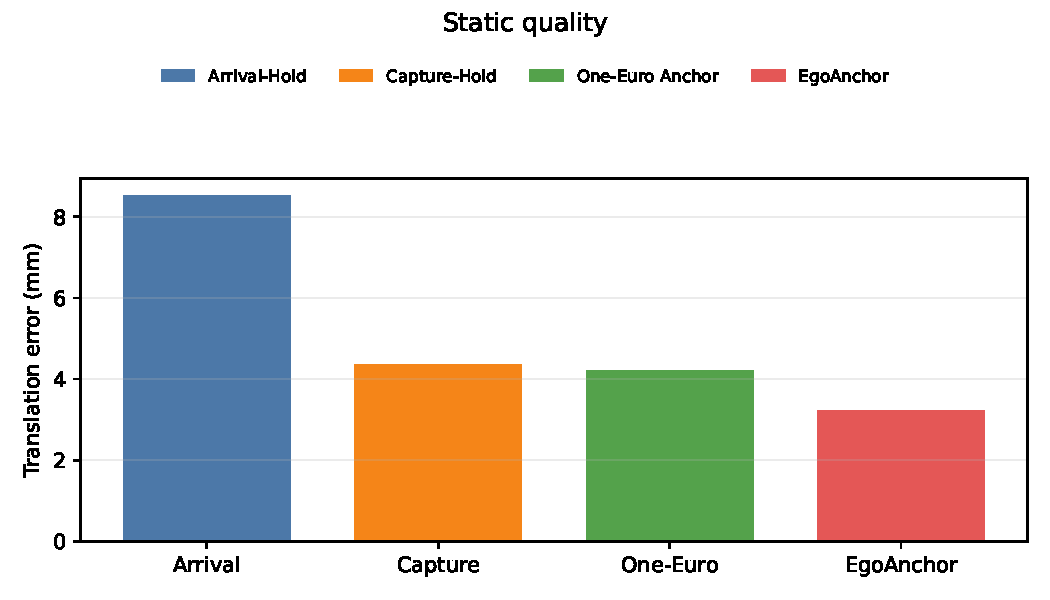
\includegraphics[width=0.32\textwidth]{figures/generated/exp1_static_timeline.pdf}
  \hfill
  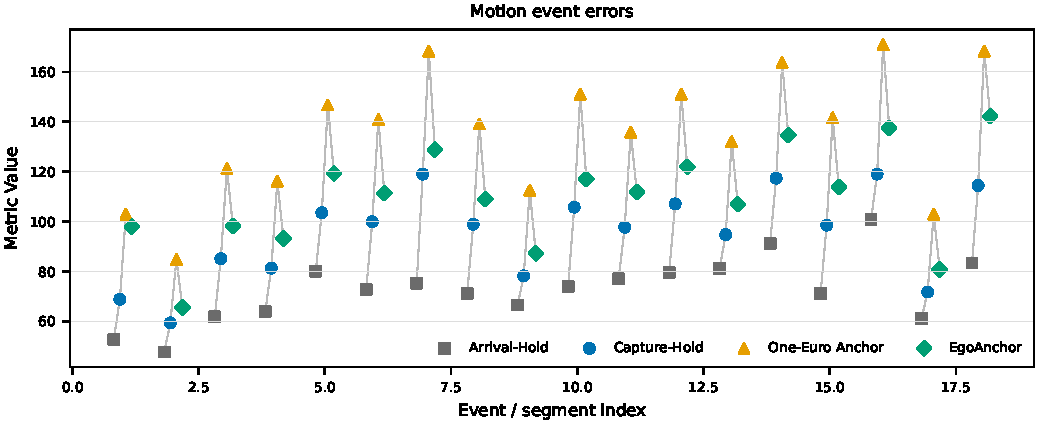
\includegraphics[width=0.32\textwidth]{figures/generated/exp1_motion_events.pdf}
  \hfill
  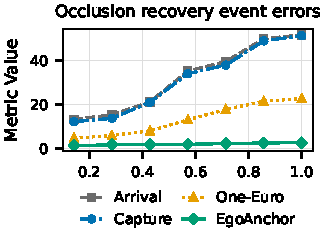
\includegraphics[width=0.32\textwidth]{figures/generated/exp1_occlusion_events.pdf}
  \caption{实验一的 event/segment 结果。左：各配置的静止头动 event 值；中：起停 6DoF 的同 event 配对；右：遮挡 event 值的经验覆盖分布。渲染 frame 不作为统计单位。}
  \label{fig:exp1-generated-events}
\end{figure*}

\subsection{实验二：系统设计归因}

实验二直接复用实验一五类物理任务的同一批候选、参考轨迹和渲染长表，不另行重复采集。正式场景在每个任务中并行运行完整 EgoAnchor 与四个单组件消融；分析阶段再按组件适用的物理场景进行逐 trial、逐事件配对。该实验不把 VCD 或静止锚定作为独立算法问题，而是检验它们是否解释端到端系统行为。

\textbf{采集时刻世界对齐。}
在静止目标与主动头动序列中比较完整 EgoAnchor 与关闭采集时刻世界对齐的变体。两种配置使用相同的 VCD 接纳、时序合成、静止锚定和生命周期管理，仅改变相机世界变换的查询时刻，并在同 event 内配对平移与旋转误差。

\textbf{VCD 观测接纳。}
在遮挡与低质量观测较多的序列上比较完整 EgoAnchor 与关闭 VCD 接纳的变体。两种配置共享相同的状态估计、时序合成和生命周期管理。候选级诊断只纳入实际到达 Unity、具有 capture-time aligned raw pose 与同帧平台参考的完整 EgoAnchor 候选；按 VCD 分数的精确 tie 阈值整体纳入，报告 mean-risk AURC 和 P95 tail-risk 曲线。VCD 在本文中被解释为锚点更新的运行时可靠性信号，而非位姿正确概率。

\textbf{时序合成。}
在起停六自由度序列中比较完整 EgoAnchor 与关闭时序合成的变体；两者保持采集时刻对齐、VCD 接纳、静止锚定和生命周期管理一致。该对比用于量化低频异步观测缺少逐帧时序合成时的连续性代价，以及显式合成在运动阶段的误差--滞后权衡。

\textbf{静止锚定。}
在静止目标与主动头动序列中比较完整 EgoAnchor 与关闭 StaticLock 的变体。两种配置共享相同的候选接纳、状态估计、插值和生命周期策略；配对指标限于位置 HP--RMS、静止漂移和绝对位姿误差，不把起停转换指标归入该消融。

\begin{table*}[t]
  \centering
  \caption{实验二单组件消融的 event-level 配对差值。差值定义为消融配置减完整 EgoAnchor；每行同时给出主指标与 guardrail。}
  \label{tab:exp2-generated-summary}
  \resizebox{\textwidth}{!}{%
% EGOANCHOR-EXP-TWO-TABLE:BEGIN
% Source CSV SHA-256: 1286cc8cc11b87b1b04a665e52f31a52cacc9880122fc3cf94d978b7cd2ff860; Stage 3 TeX SHA-256: 988c40fa4959382332ed659549101acff503ccf903c1f43c5c340dbbf0ea3eb9; generator: egoanchor.eval.materialize-v1; file: exp2_tables.tex
% 由 egoanchor.eval 自动生成，请勿手工修改本区块。
% Table: exp2\_component\_deltas
\begin{tabular}{llllllll}
\toprule
结果 & 消融配置 & 场景 & 主指标 & 主差值 [IQR] & 护栏指标 & 护栏差值 [IQR] & 配对数 \\
\midrule
采集时刻对齐 & 关闭采集时刻对齐 & 静止头动 & 平移误差 event-P95 & 5.585 [0.6, 13.959] mm & 旋转误差 event-P95 & 0.41 [0.216, 0.813] deg & 4/4 \\
VCD 接纳 & 关闭 VCD & 遮挡恢复 & 遮挡窗平移 P95 & 21.857 [0, 46.254] mm & 持久恢复时间 & 0 [0, 0] ms & 7/7 \\
时序合成 & 关闭时序合成 & 起停 6DoF & 平移跳变 P95 & -1.736 [-2.72, -0.54] mm & 可见响应时间 & 0 [0, 0] ms & 5/5 \\
StaticLock & 关闭 StaticLock & 静止头动 & 位置 HP-RMS & 1.592 [0.959, 2.205] mm & 绝对平移误差中位数 & 1.197 [1.063, 1.491] mm & 4/4 \\
\bottomrule
\end{tabular}
% EGOANCHOR-EXP-TWO-TABLE:END
  }
\end{table*}

表~\ref{tab:exp2-generated-summary} 汇总了三个适用场景中的同 event 配对。关闭采集时刻对齐后，静止头动平移 event-P95 的中位差值为 $\EAExpTwoCaptureTimeAlignmentTranslationEventPNinetyFiveMmDeltaMedian$~mm；关闭 StaticLock 后，位置 HP--RMS 的中位差值为 $\EAExpTwoStaticLockPositionHpRmsMmDeltaMedian$~mm。两项在本批次配对事件中均为正值。关闭 VCD 后，遮挡窗平移 P95 的中位差值为 $\EAExpTwoVcdAdmissionOcclusionTranslationPNinetyFiveMmDeltaMedian$~mm。$\EAExpTwoVcdMeanRiskCandidateCount$ 个 eligible candidate 的 VCD mean-risk AURC 为 $\EAExpTwoVcdMeanRiskAurcMm$~mm，随机顺序参考为 $\EAExpTwoRandomMeanRiskAurcMm$~mm；该比较只说明本对象、本次遮挡协议中的候选风险判别性。

时序合成呈现混合的尾部权衡。关闭该组件后，平移跳变 P95 的中位差值为 $\EAExpTwoTemporalSynthesisJumpPNinetyFiveMmDeltaMedian$~mm，P99 差值为 $\EAExpTwoTemporalSynthesisJumpPNinetyNineMmDeltaMedian$~mm，可见响应时间差值为 $\EAExpTwoTemporalSynthesisVisibleResponseMsDeltaMedian$~ms。P95 与 P99 方向相反，不能据此概括为单一净收益；持续运动中的误差--时延关系仍以实验一分场景结果为准。

\begin{figure*}[t]
  \centering
  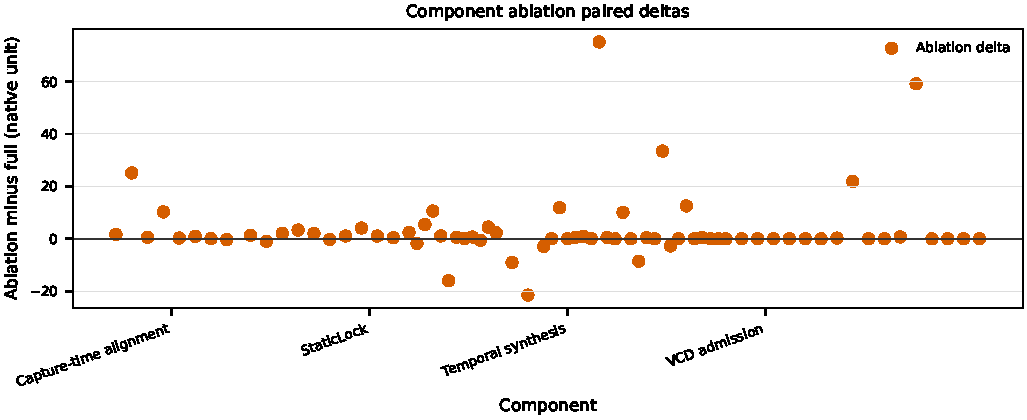
\includegraphics[width=0.48\textwidth]{figures/generated/exp2_component_deltas.pdf}
  \hfill
  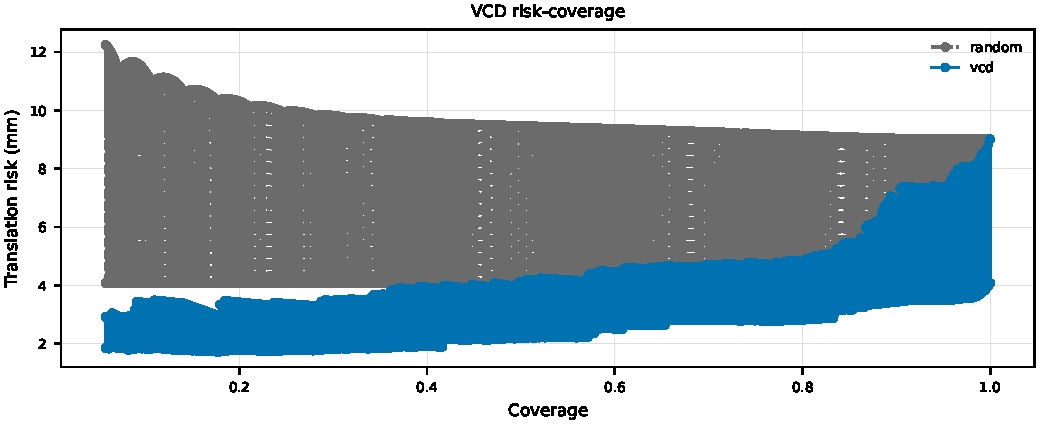
\includegraphics[width=0.48\textwidth]{figures/generated/exp2_vcd_curve.pdf}
  \caption{实验二的组件配对差值与 VCD 候选级 P95 tail-risk 曲线。差值为消融配置减完整 EgoAnchor；曲线基于 $\EAExpTwoVcdMeanRiskCandidateCount$ 个 risk-eligible、实际到达 Unity 的完整 EgoAnchor 候选，仅作描述性诊断。}
  \label{fig:exp2-generated-summary}
\end{figure*}

\subsection{评价指标与汇总}

所有序列均以 display pose 相对于同一 Quest 平台参考的平移和旋转误差为基础。静止头动报告绝对误差、漂移与高通 RMS；起停序列报告运动窗误差、峰值误差、跳变、可见响应和重新稳定时间；遮挡序列分别在遮挡窗与重新可见后的恢复窗计算误差、更新和持久恢复指标。

持续运动的\emph{有效时延}在每个 event 内通过冻结 lag 网格搜索得到：平移通道最小化 $\mathrm{display}(t)$ 与 $\mathrm{reference}(t-\mathrm{lag})$ 的 RMSE，旋转通道最小化对应角残差，并要求满足连续区间和最小重叠契约。该量是相对于平台参考轨迹的描述性拟合时延，不等同于视觉候选的网络到达时延或运行时主动设置的插值延迟。VCD risk--coverage 是候选级评分诊断，独立于 event-level 系统比较，不用于候选级显著性推断。

各指标首先在每个预定义事件或试次内计算，再在对应长序列中汇总。我们报告描述性统计和同一事件内的方法配对差异。渲染帧用于形成连续轨迹，不作为独立统计样本，也不进行帧级显著性检验。

\subsection{实验三：跨对象用户研究计划}

实验三用于检验系统差异是否能转化为对象附着型 MR 任务中的表现与体验收益。该实验将在实验一和实验二完成并冻结系统参数后启动；当前阶段只固定研究设计、伦理材料、任务流程与日志接口，不纳入本轮正式采集和结果报告。

用户研究拟采用被试内设计，比较 \emph{One-Euro Anchor} 与完整 EgoAnchor，并覆盖无线鼠标、带柄杯和纯色盒体三个日常刚性物体。三者分别代表中等纹理的小型曲面、弱纹理且易受抓握遮挡的局部非对称几何，以及低纹理的多平面几何。方法顺序在参与者之间平衡，任务顺序和对象顺序采用平衡随机化；相同对象在两种方法下使用难度匹配但内容不同的标签和目标，以降低记忆效应。

\textbf{移动与观察。}
参与者拿起目标物体，将其移动至指定区域并按照提示旋转，以寻找附着于不同表面的虚拟标签。该任务测量运动期间的连续附着、停止后的稳定性和对象附着信息的可读性。主要客观指标为信息识别错误；次要指标包括完成时间和额外物体调整次数。

\textbf{遮挡、恢复与选择。}
参与者观察附着于物体的虚拟控制面板，按照提示将目标置于标准遮挡区域并保持 2--3~s，随后将其移回可见区域并选择指定的对象附着控件。该任务测量重新可见后的锚点恢复、恢复后的虚实对齐以及用户对恢复行为的信任。主要客观指标为错误选择次数和目标重新可见至首次成功选择的时间；次要指标包括重试次数和需要实验员干预的失败次数。

主观指标包括七点量表上的感知锚点稳定性、响应性、恢复后对齐和信任；NASA-TLX 在每个方法条件完成后填写，总体偏好在全部条件结束后记录。参与者数量初步按 18--20 人规划，最终样本量依据相关研究中的效应量和预先设定的统计功效完成先验功效分析后确定。


\section{讨论与局限}\label{sec:discussion}


\subsection{设计启示}


EgoAnchor 将异步视觉观测转换为对象锚点时，需要区分相机运动造成的坐标变换错配与目标物体在观测到达前继续运动造成的轨迹滞后。基于帧标识的采集时刻对齐处理前一问题；运动估计与时序平滑只在观测之间维持连续输出，并不消除采集后的目标运动滞后。两类误差具有不同的时间语义，不能由单一“端到端时延”指标替代。

\textbf{时间一致性的边界。} 帧对齐可避免将历史相机系观测与到达时刻相机位姿错误复合，但不能恢复目标物体在采集之后的当前位姿。动态场景仍受感知处理时间、观测更新率和平滑策略引入的插值延迟共同影响。因此，动态表征以渲染时刻误差描述应用实际获得的配准质量，不把帧对齐表述为对物体运动时延的补偿。

\subsection{平台定位与可比性}

平台原生对象追踪、商业模型目标系统与物体侧专用追踪器为动态物体关联提供了不同路径，但它们并不是 EgoAnchor 观测到锚点运行时的同任务算法基线。不同方案在支持对象、模型或标记准备、传感器硬件、内部候选可见性、预测与平滑策略以及输出坐标语义上均可能不同。跨设备数值对比会把这些因素与运行时设计混合在一起，因此本文通过相关工作与能力表说明其适用边界，并将核心定量比较限制在同一 Quest、同一视觉候选流、同一平台参考和同一时间线下的系统配置与组件消融。只有当两个系统支持同一物理对象、能够执行同一动作并具有独立共同参考时，平台对比才适合作为描述性的部署案例，而不用于支撑本文的核心机制主张。

\subsection{局限与未来工作}


EgoAnchor 面向具有可用三维模型的刚性物体，其对象类别不由预定义标签集限制，新的刚性目标可在无需逐物体训练的情况下接入同一系统。实际锚定质量仍取决于物体在头显图像与双目深度中的可观测性：严重遮挡、极弱纹理、透明或镜面材质以及超出有效深度量程都会削弱分割、几何重建和位姿验证。非刚性物体需要可变形表示与非刚体跟踪，超出本文采用的刚体位姿模型。缺少现成三维模型时，Image-to-3D 重建可以补充模型来源，但重建误差会传递至锚定结果。受控定量评价使用 Quest 控制器的平台位姿，因此无法观测平台参考与头显之间共同的世界系漂移，也不能排除参考轨迹自身的预测、平滑与动态时延；文中误差应理解为平台参考下的相对误差，而非外部光学系统给出的物理真值。每类定量场景仅由一条包含重复事件的长序列表征，因而主要支持配对的系统行为分析。实验三尚处于计划阶段，日常物体上的任务效用与跨对象泛化仍需在后续用户研究中完成验证。系统当前还依赖外部 GPU 工作站，部署成本与网络条件构成进一步的应用约束。

未来工作将探索更广的物体覆盖、对非刚性物体的支持，以及与生成式三维重建的更紧密结合。

\section{结论}\label{sec:conclusion}

本文提出 EgoAnchor，一套面向消费级混合现实的端到端动态真实物体锚定系统。系统以头戴显示器双目图像和目标物体的可用三维模型为输入，通过视觉感知后端与对象锚定运行时的分层架构，将历史采集时刻、低频且质量不均的相机系位姿观测转换为应用可持续消费的世界系对象锚点。EgoAnchor 通过采集时刻世界对齐恢复异步观测的时间语义，通过 VCD 观测接纳限制有害更新，并以连续时序合成、显式静止锚定和生命周期管理定义静止、运动、短时失效与恢复期间的输出行为。本文据此把零样本对象感知与混合现实应用之间的接口问题明确为一项系统设计任务，并通过具有平台参考的端到端系统表征和关键组件消融评价其系统能力与应用边界。


\bibliographystyle{abbrv-doi-hyperref-narrow}
\bibliography{egoanchor_cn_refs}

\end{document}
